%===================================== CHAP 4 =================================

\chapter{Experiments and results}\label{chpt:experiments}

Due to the initial discussion that arose related to synchronicity in the CA3-layer of the model after other model decisions had been made, and a working and debugged model had been attained, initial experiments are going to be performed on a novel synchronous versus asynchronous model. From these findings, the model attaining the best performance will be used in further experiments. In the event of similar results, the most algorithmically efficient model will be preferred, which would be the synchronous updating scheme.

Following the preliminary study on synchronicity is the extended preliminary experimentation on model calibration, in which I search to attain a good model configuration. The attained parametrization will then be employed in the experiments replicated from \citep{Hattori2014}. Results will then form a basis for a comparative analysis between the former model and the model of this thesis. 
This may lay the foundation for constructing novel experiments, testing aspects related to convergence criteria, data set dimensionality, generalisability and network design.

\section{Setup}

Using the synchronous updating scheme of CA3, the initial setup which was used was the following. The dimensionality was as specified in the previous chapter, having the input and outputs dimensions consist of $49$ neurons in the main extraction experiments. As for the EC-, DG-, and CA3-layers, these consist of a different number of neurons, see table \ref{table:number_of_neurons}. Furthermore, their firing rates were set accordingly as in \citep{Hattori2014}, see table \ref{table:firing_rates}.

\begin{table}[]
\centering
\caption{Lists the number of neurons in each layer within the hippocampal module.}
\label{table:number_of_neurons}
\begin{tabular}{l|l|l|l|l|l|}
\cline{2-6}
                              & Input & EC  & DG   & CA3 & Output \\ \hline
\multicolumn{1}{|l|}{Neurons} & 49    & 240 & 1600 & 480 & 49     \\ \hline
\end{tabular}
\end{table}

\begin{table}[]
\centering
\caption{Displaying the firing rates for the different layers, and the resulting values $k$ for k-Winners-Takes-All.}
\label{table:firing_rates}
\begin{tabular}{l|l|l|l|}
\cline{2-4}
                                  & EC   & DG   & CA3  \\ \hline
\multicolumn{1}{|l|}{Firing rate} & 0.10 & 0.01 & 0.04 \\ \hline
\multicolumn{1}{|l|}{Resulting $k$} & 24 & 16 & 19 \\ \hline
\end{tabular}
\end{table}

Lastly, the neuronal turnover rate, together with the weighting of the connections from DG during learning, were parameters that were calibrated during preliminary of experiments. The data which was empirically obtained are presented below in chapter \ref{section:experiments}. Initially, the parametrization of the model settings was as presented in table \ref{table:initial_settings}, the DG-weighting being set to $25.0$, and the neuronal turnover rate to $0.50$.

\begin{table}[]
\centering
\caption{Initial model settings for the listed parameters. Neuronal turnover was calibrated through initial experiments along with the CA3 neuronal updating scheme and DG-weighting.}
\label{table:initial_settings}
\begin{tabular}{|l|l|l|l|l|l|l|l|l|l|}
\cline{1-8}
Parameter: & Gamma & Epsilon & Nu   & k\_m & k\_r & a\_i & alpha \\ \hline
Value:     & 0.70  & 100.0   & 0.10 & 0.10 & 0.95 & 0.80 & 2.00 \\ \hline
\end{tabular}
\end{table}


% ========================== EXPERIMENTS ============================          
\section{Experiments}\label{section:experiments}

\subsection{Experiment 1: The updating scheme of CA3 and Neuronal Turnover}
\subsubsection{Synchronous updating}

\begin{figure}[h!]
    \centering
    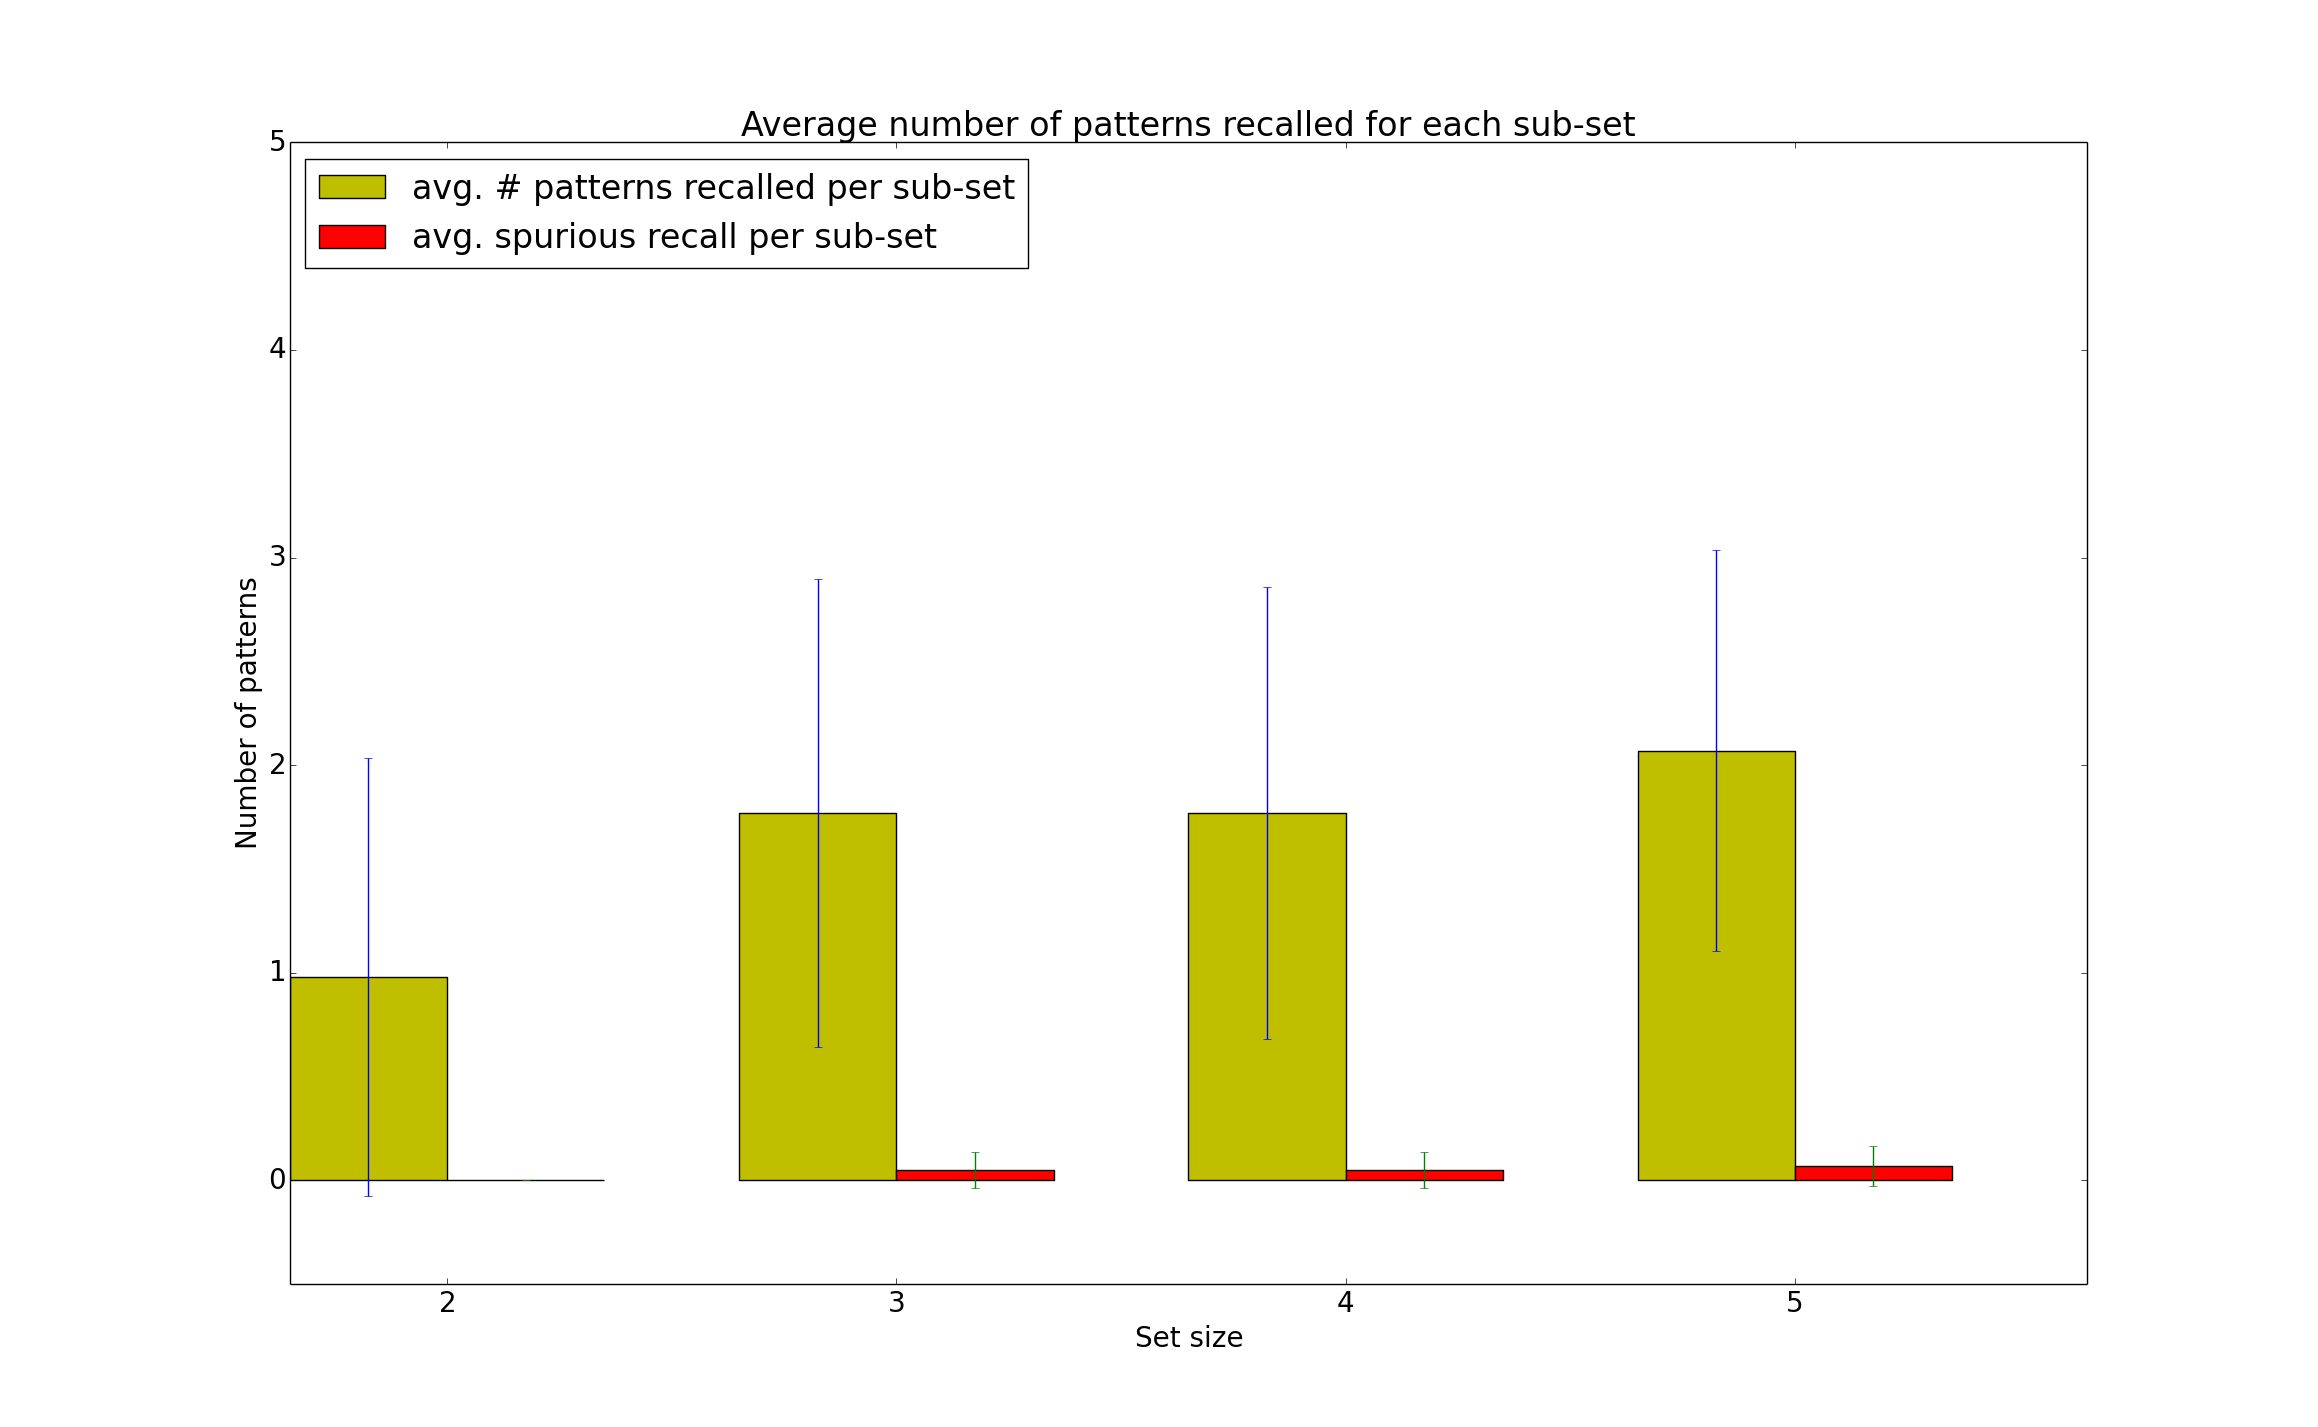
\includegraphics[width=13cm]{fig/async_false_mode_0.png}
    \caption{async false mode 0}
    \label{fig:async_false_mode_0}
\end{figure}

\begin{figure}[h!]
    \centering
    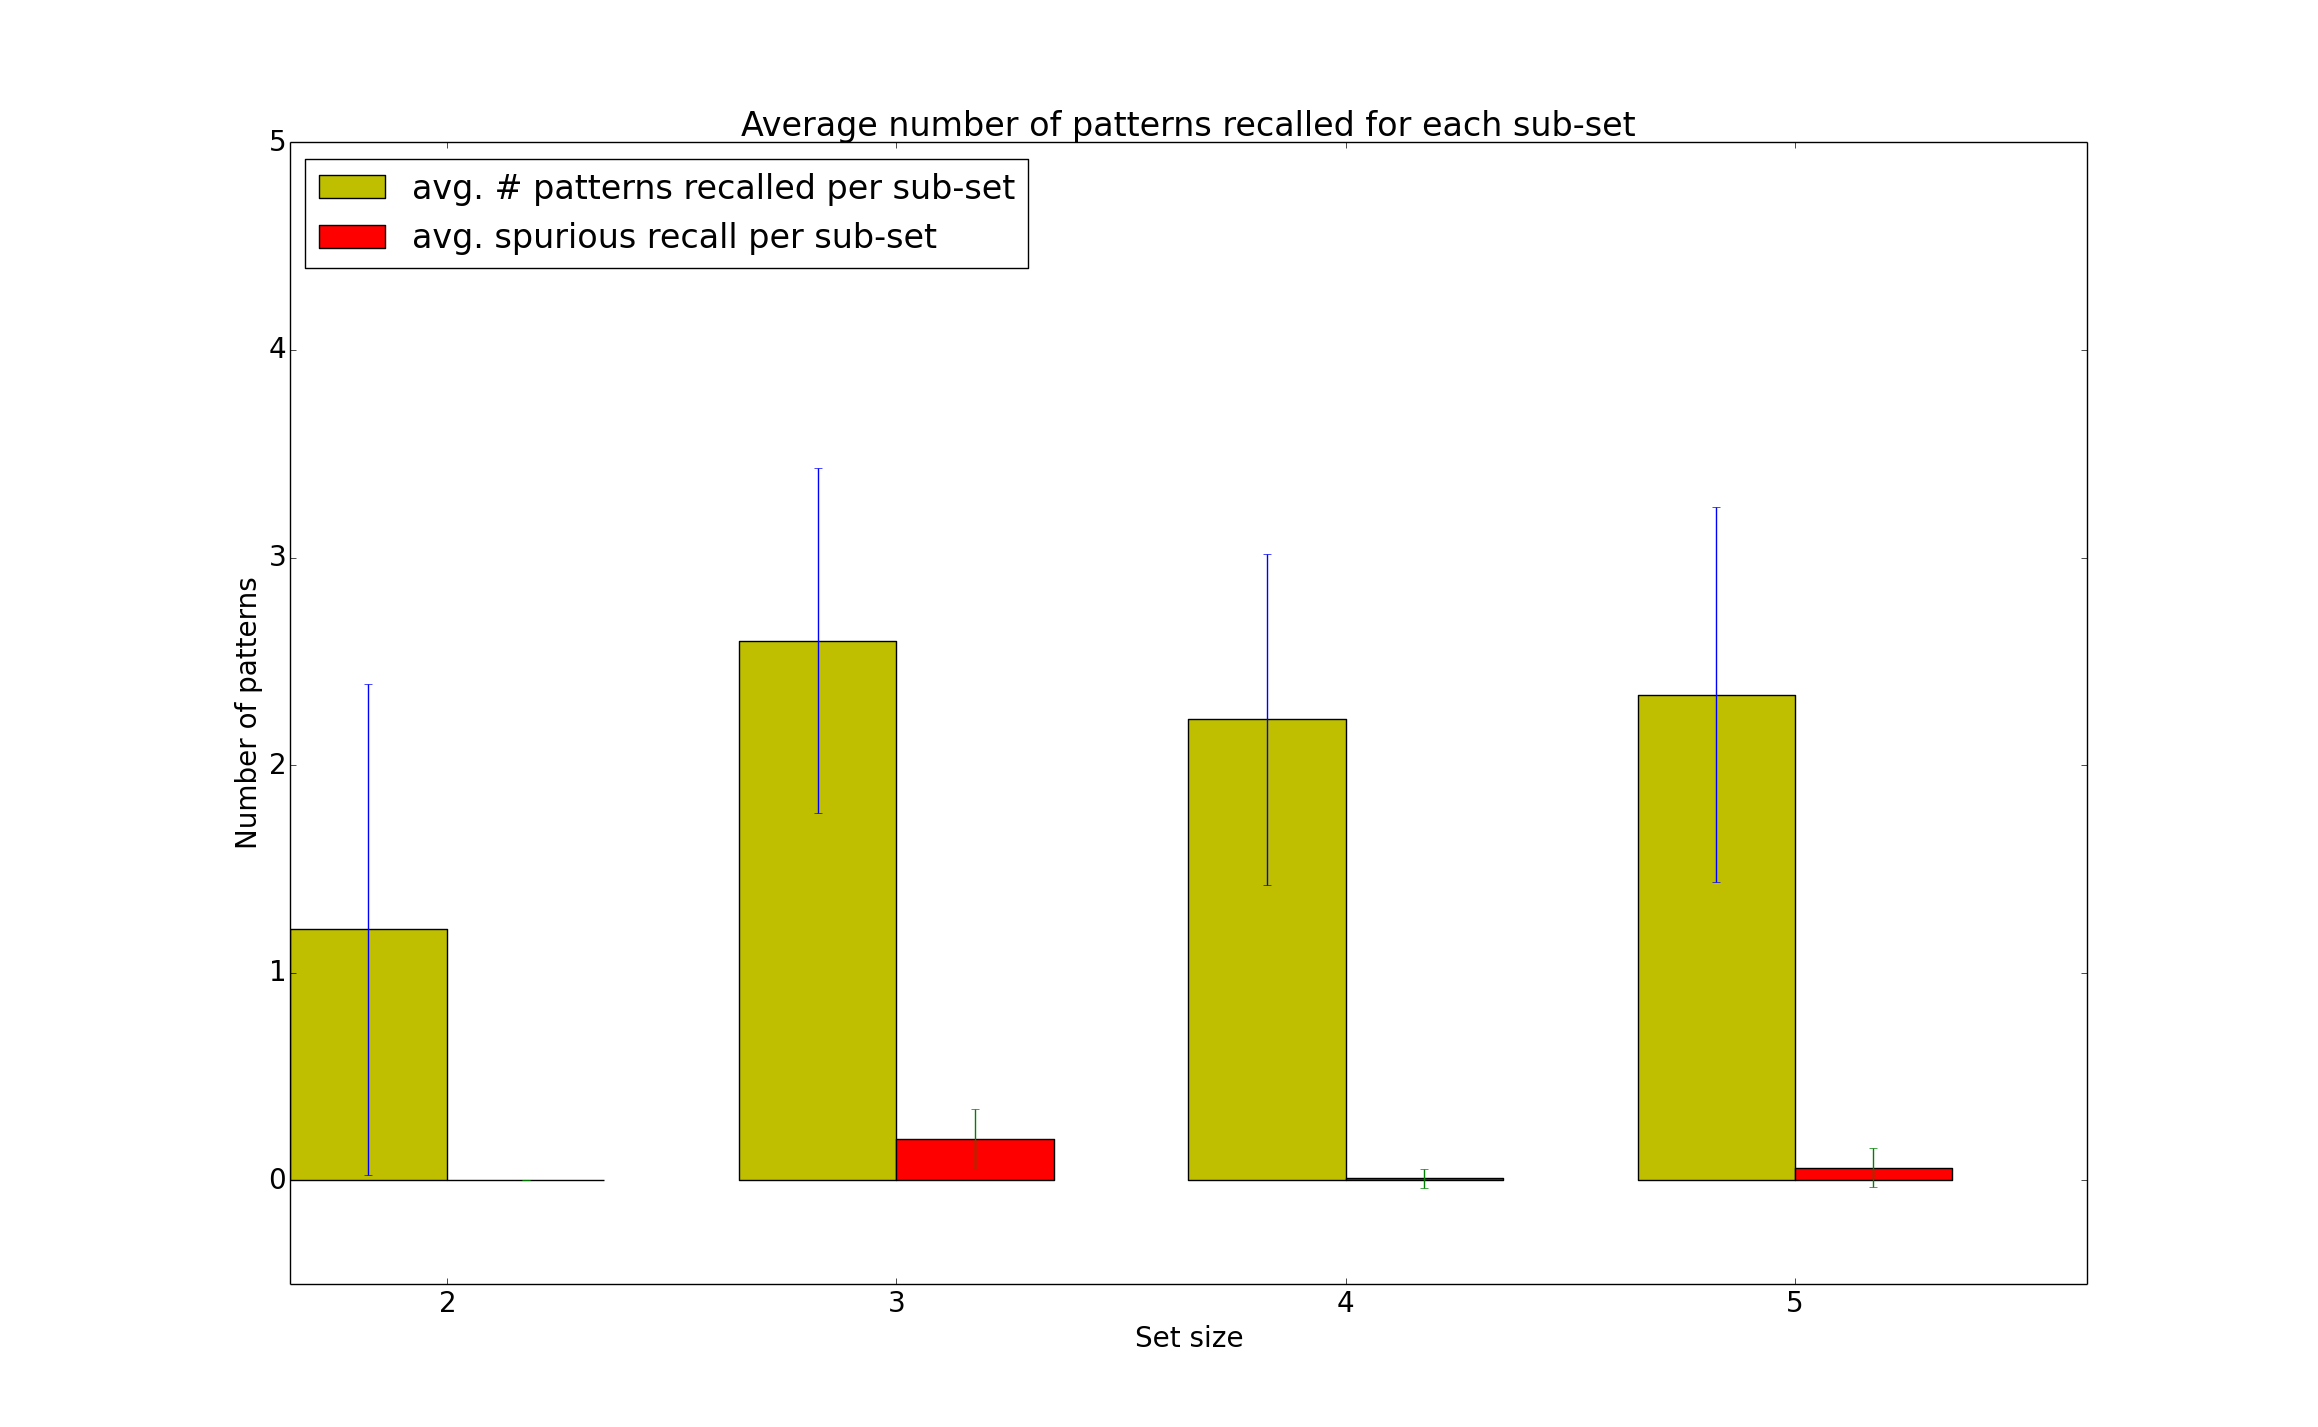
\includegraphics[width=13cm]{fig/async_false_mode_1.png}
    \caption{async false mode 1}
    \label{fig:async_false_mode_1}
\end{figure}

\subsubsection{Asynchronous updating}

\begin{figure}[h!]
    \centering
    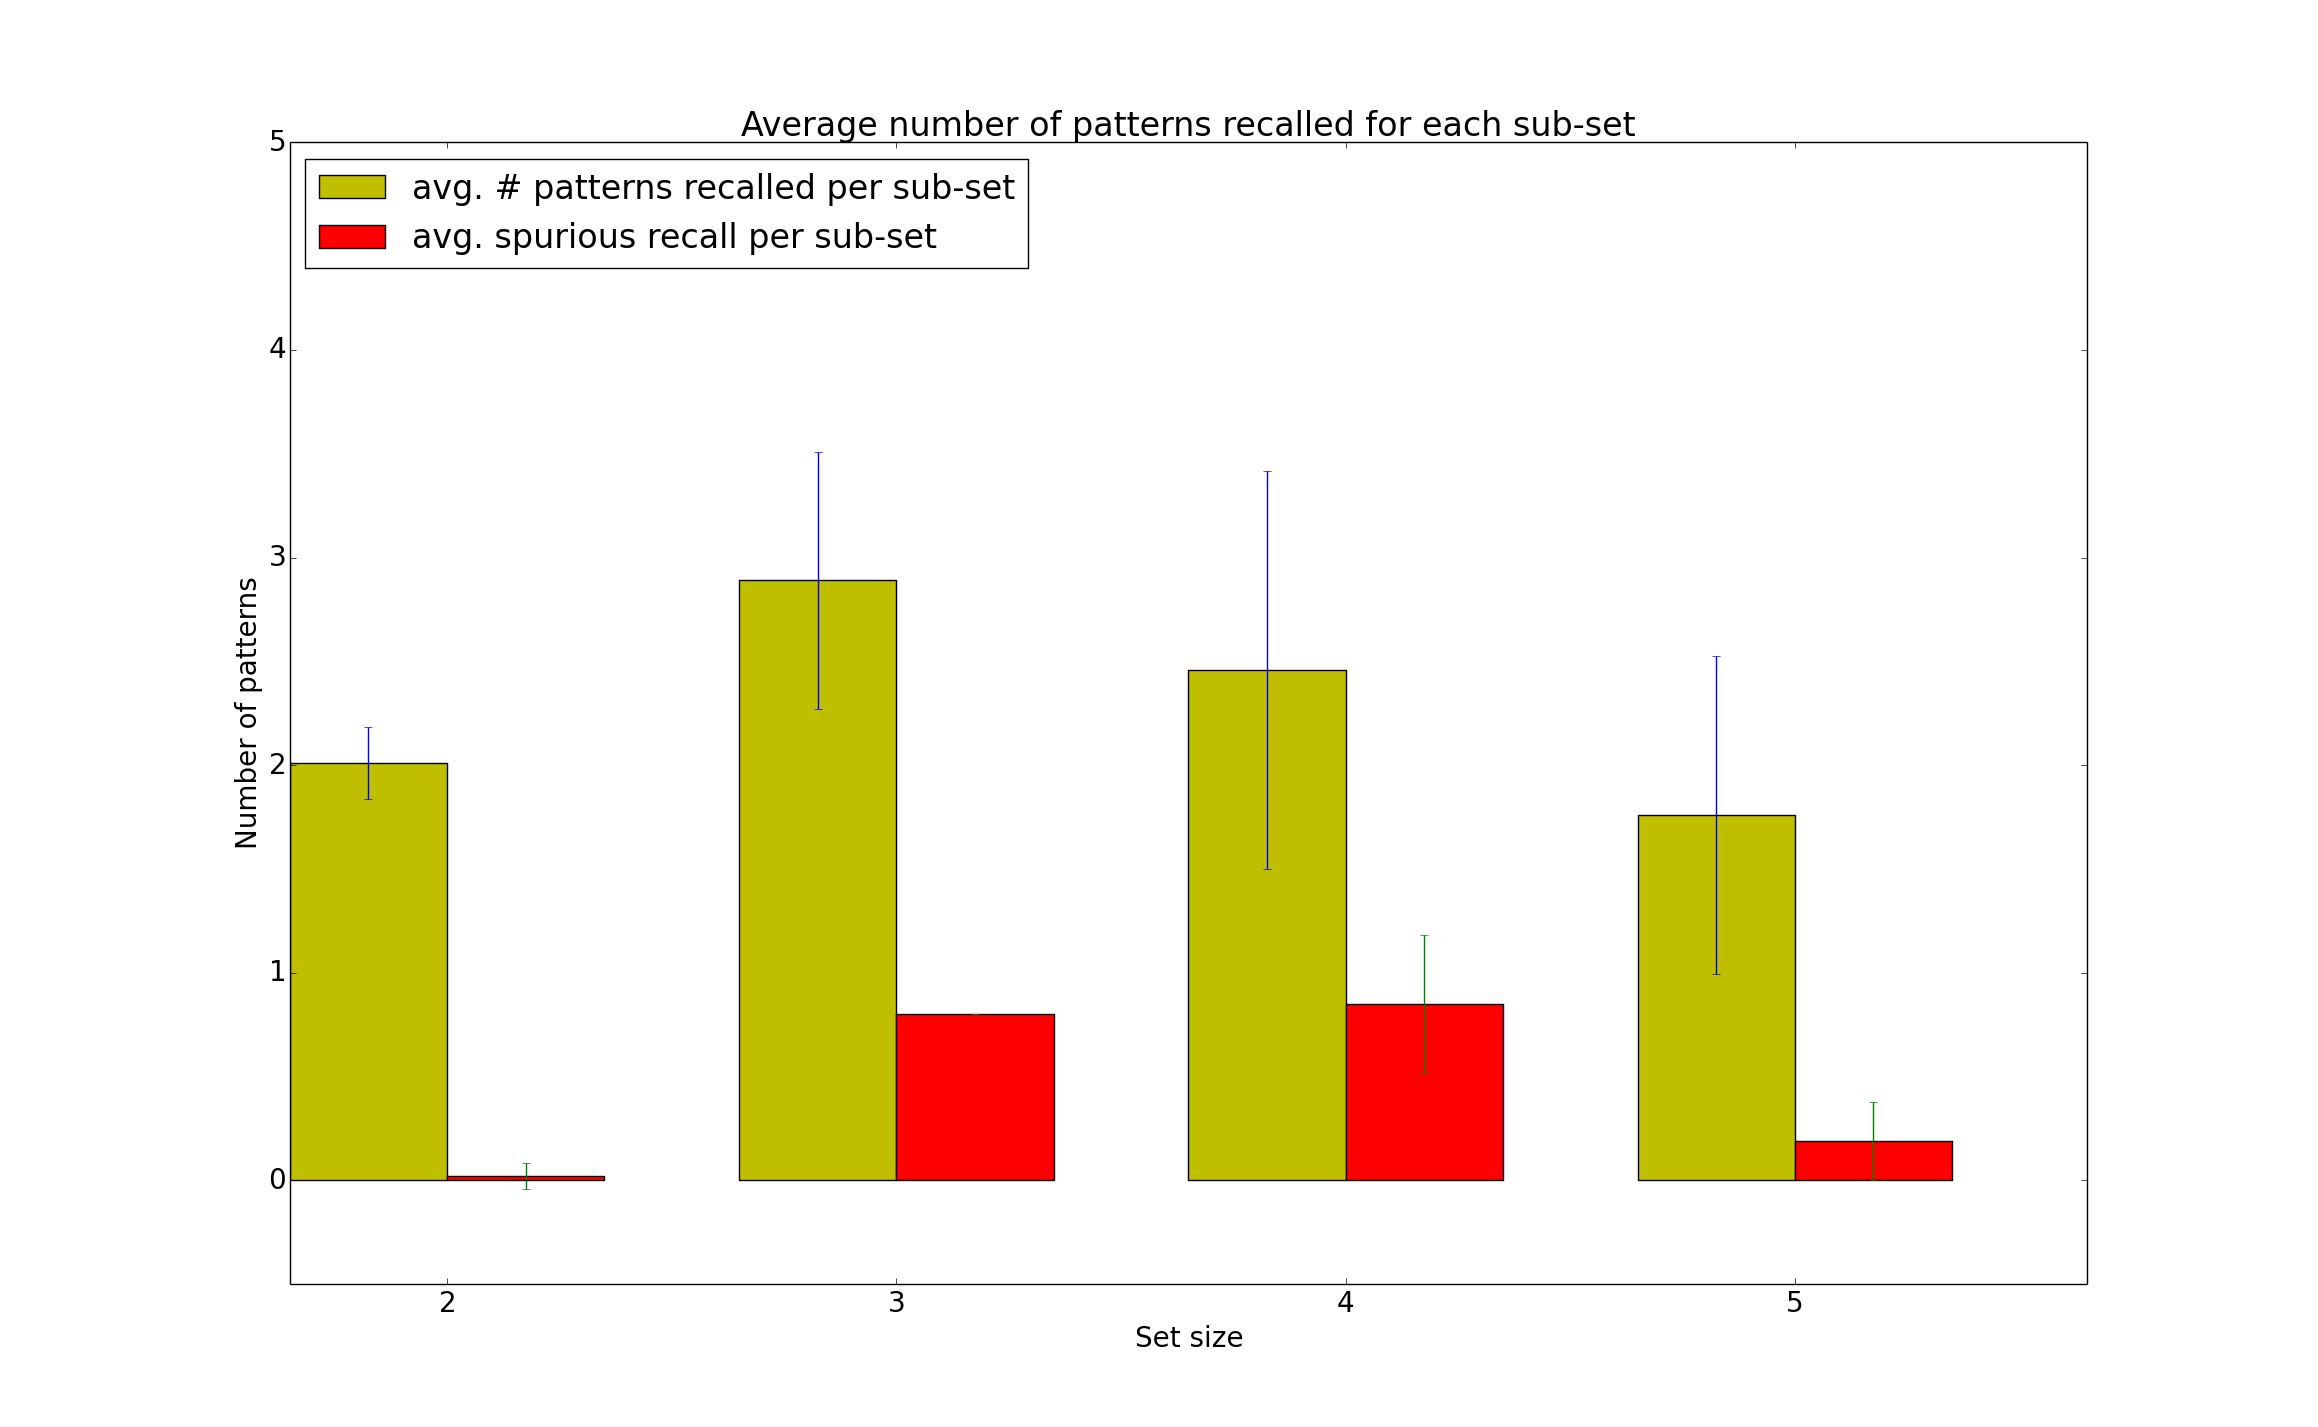
\includegraphics[width=13cm]{fig/async_true_mode_0.png}
    \caption{async true mode 0}
    \label{fig:async_true_mode_0}
\end{figure}

\begin{figure}[h!]
    \centering
    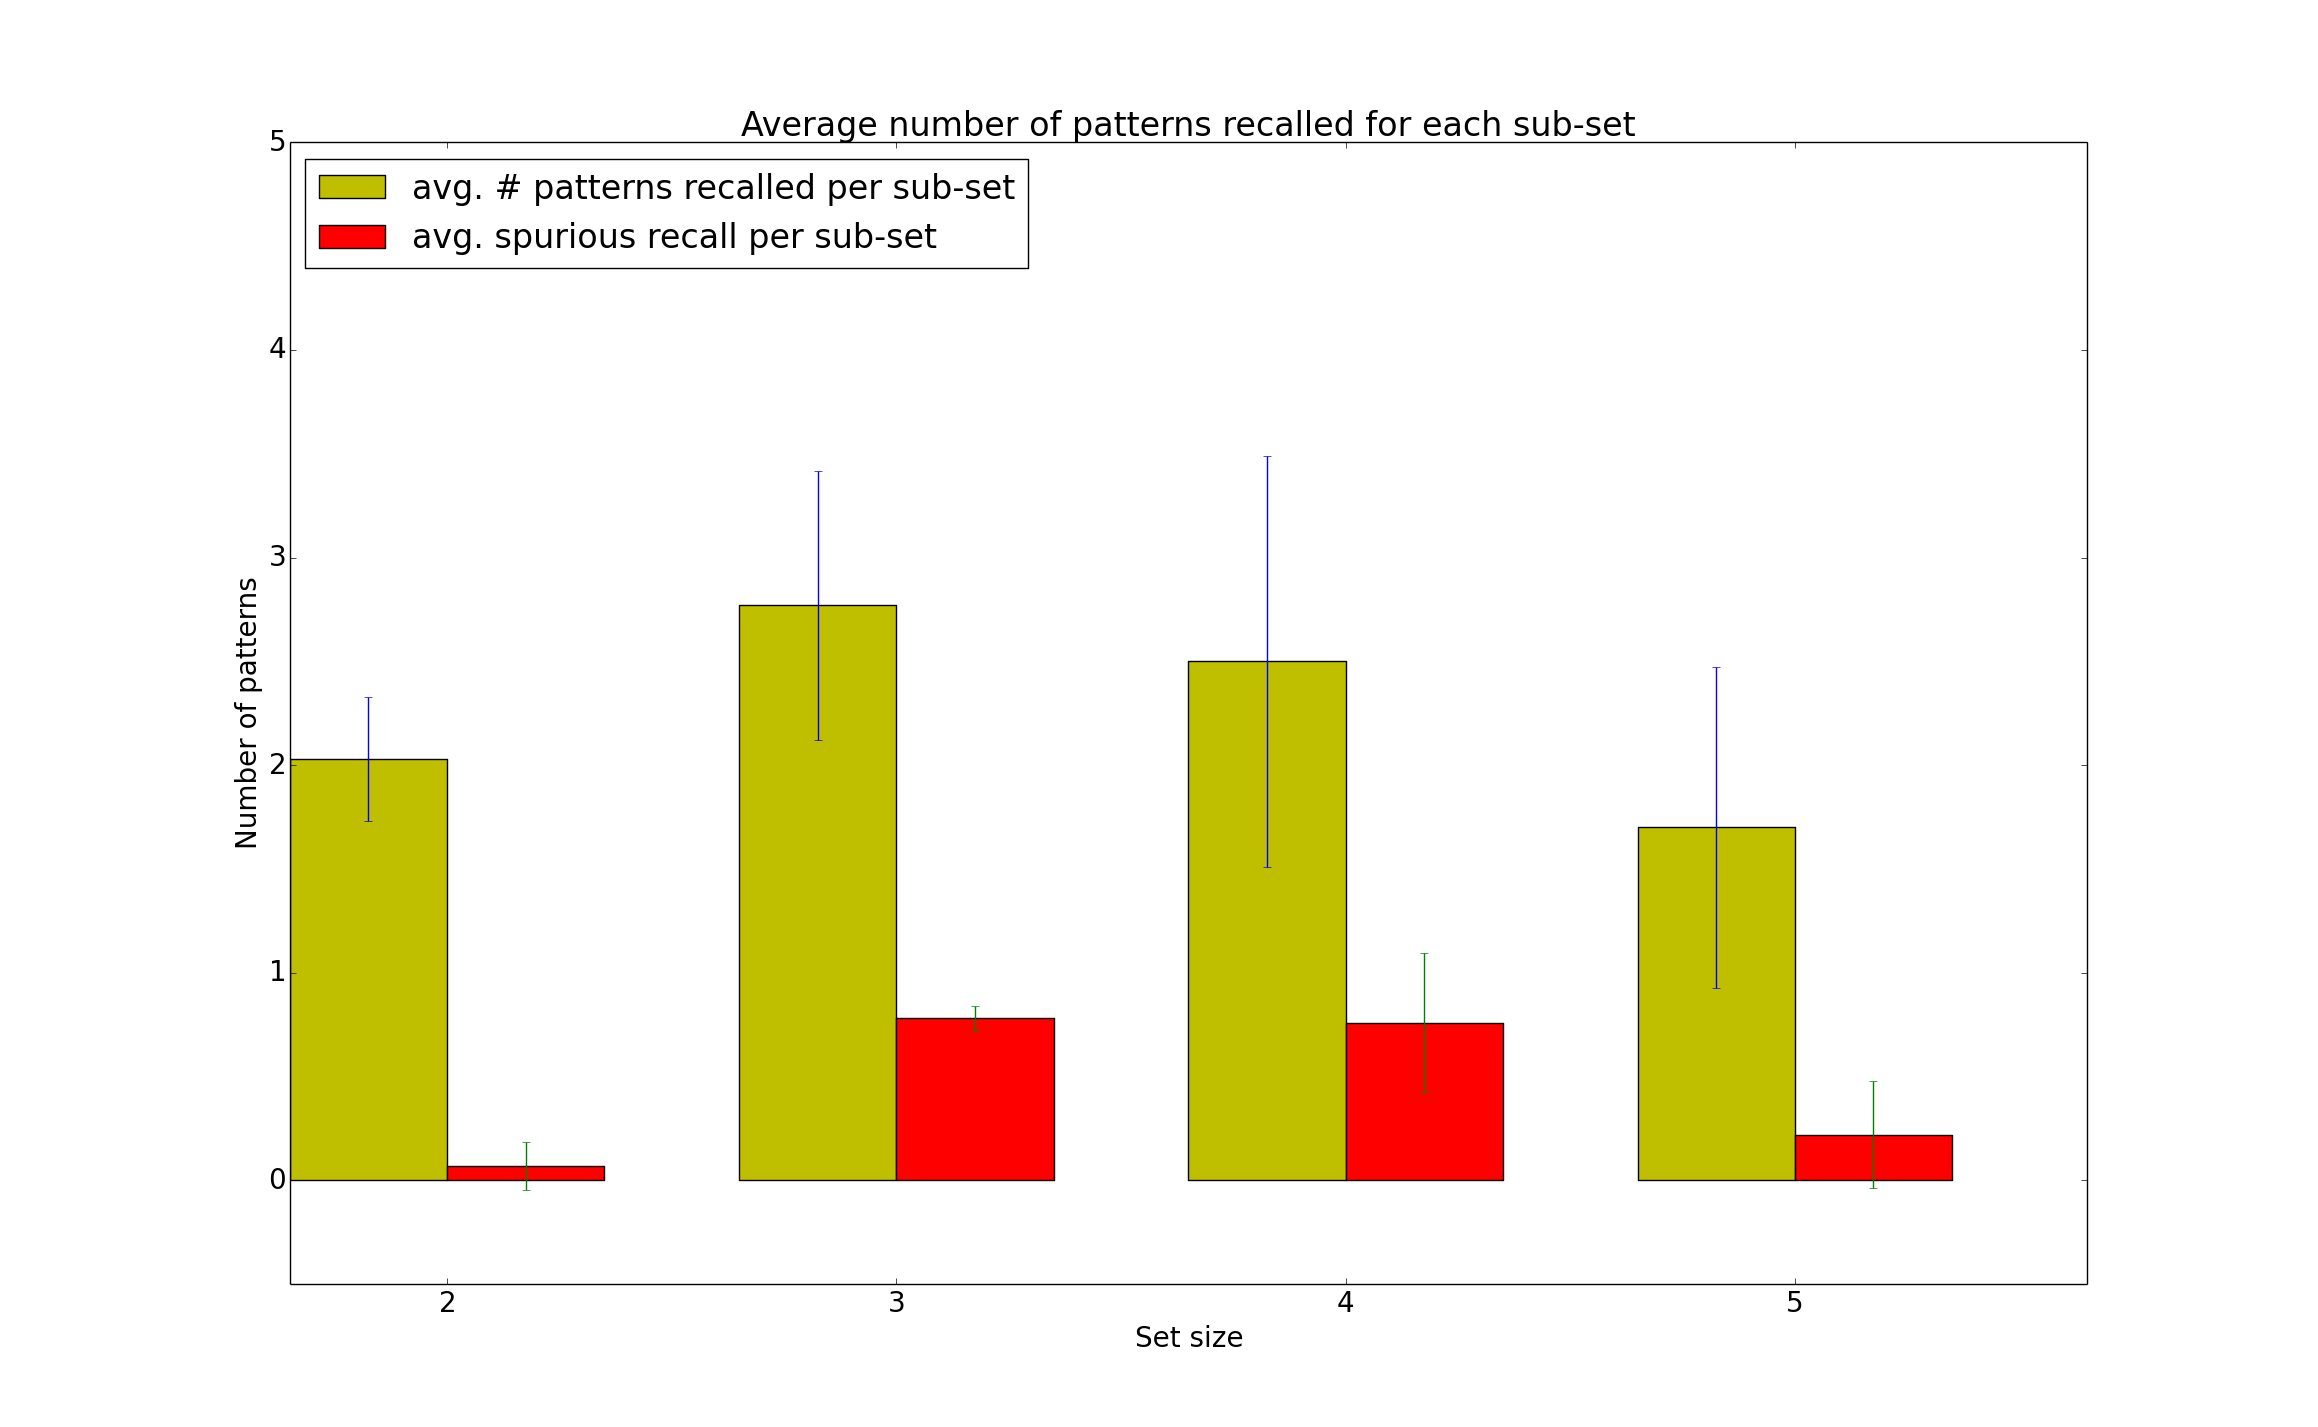
\includegraphics[width=13cm]{fig/async_true_mode_1.png}
    \caption{async true mode 1}
    \label{fig:async_true_mode_1}
\end{figure}

% ========= for all ==========
\begin{figure}[h!]
    \centering
    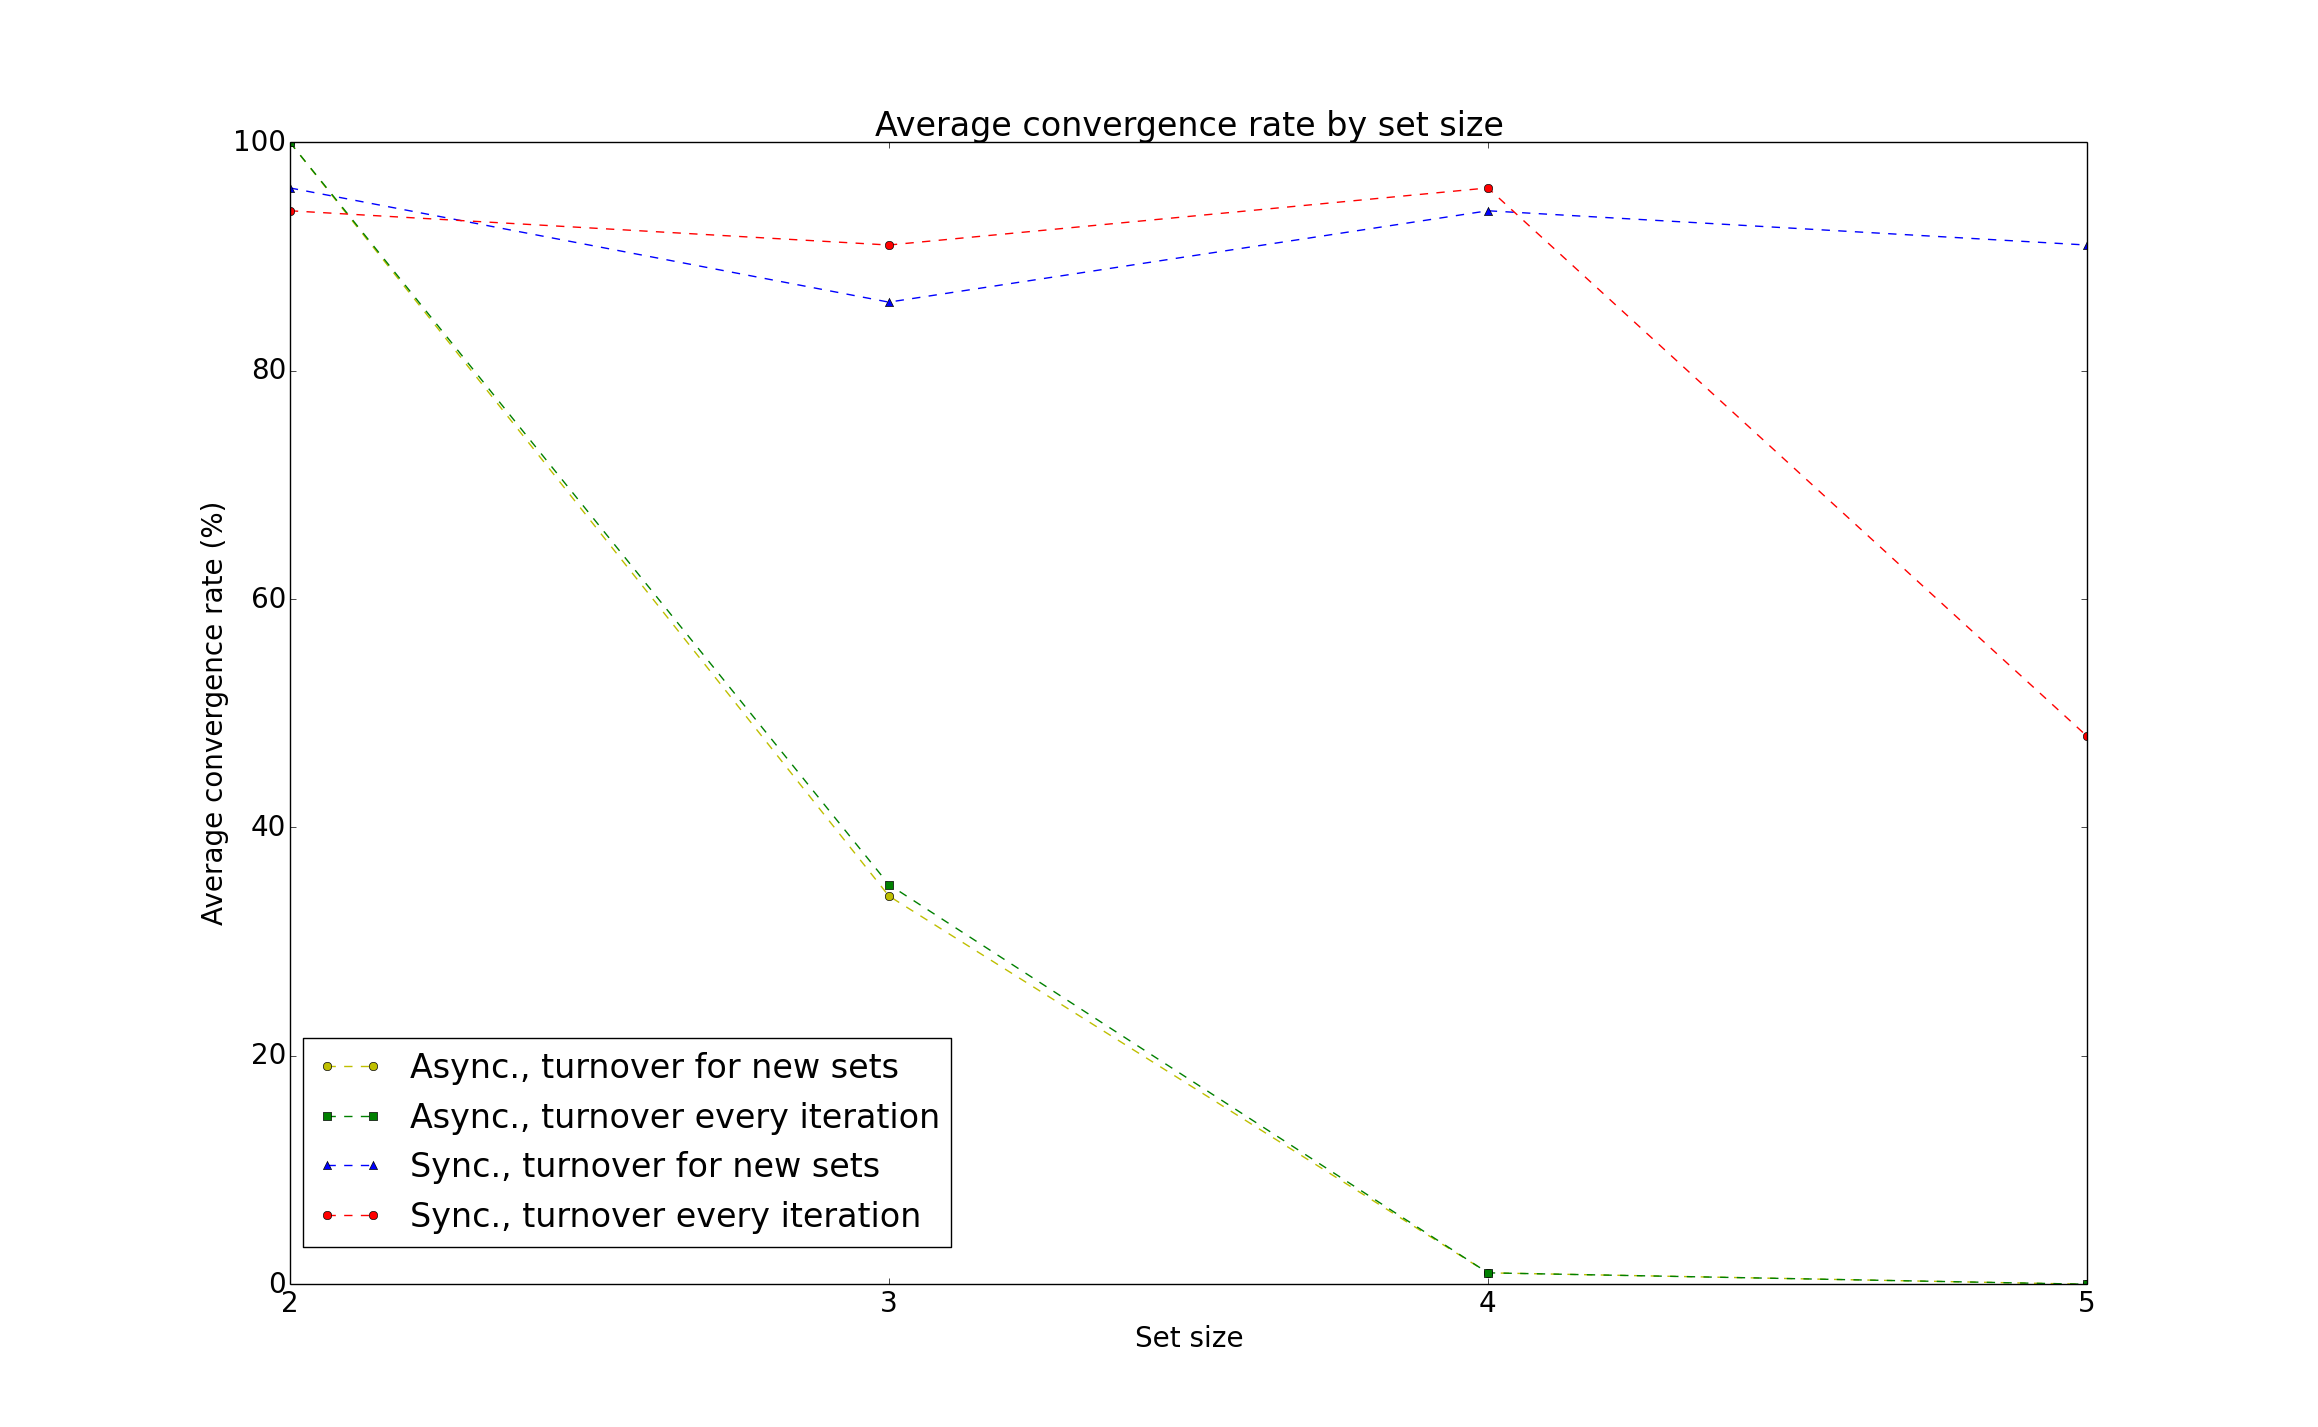
\includegraphics[width=13cm]{fig/avg_convergence_rate.png}
    \caption{avg convergence by set size}
    \label{fig:avg_convergence_rate}
\end{figure}

\begin{figure}[h!]
    \centering
    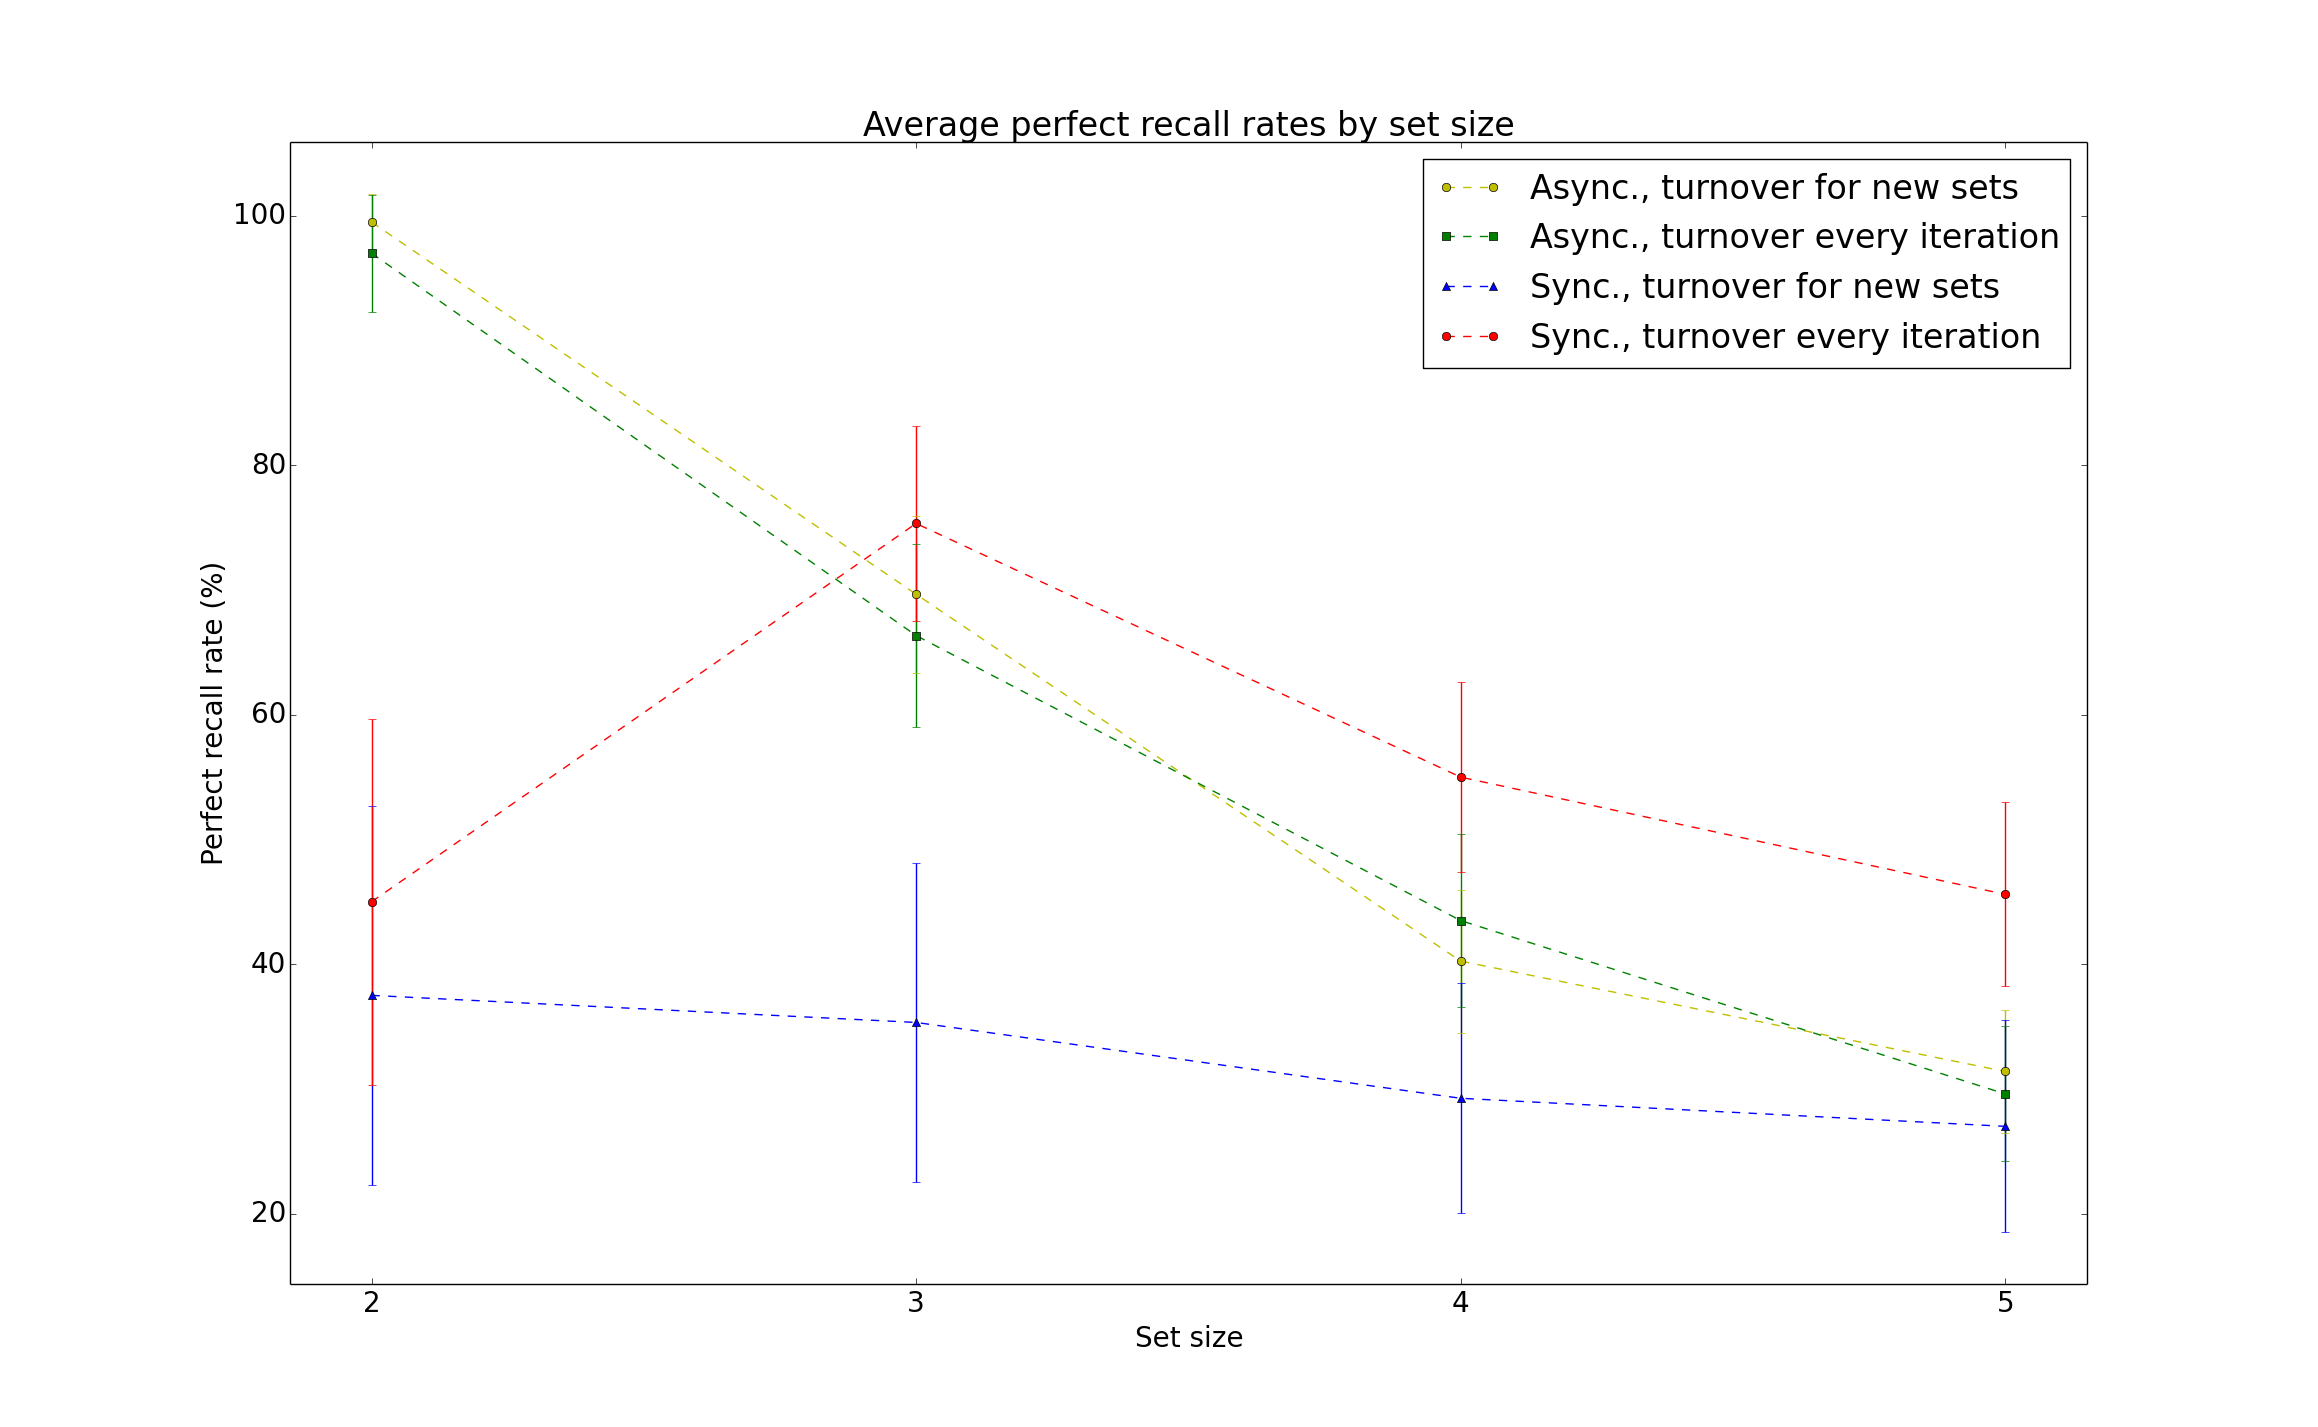
\includegraphics[width=13cm]{fig/avg_perfect_recall_rates.png}
    \caption{perf recall by set size}
    \label{fig:avg_perfect_recall_rates}
\end{figure}

\begin{figure}[h!]
    \centering
    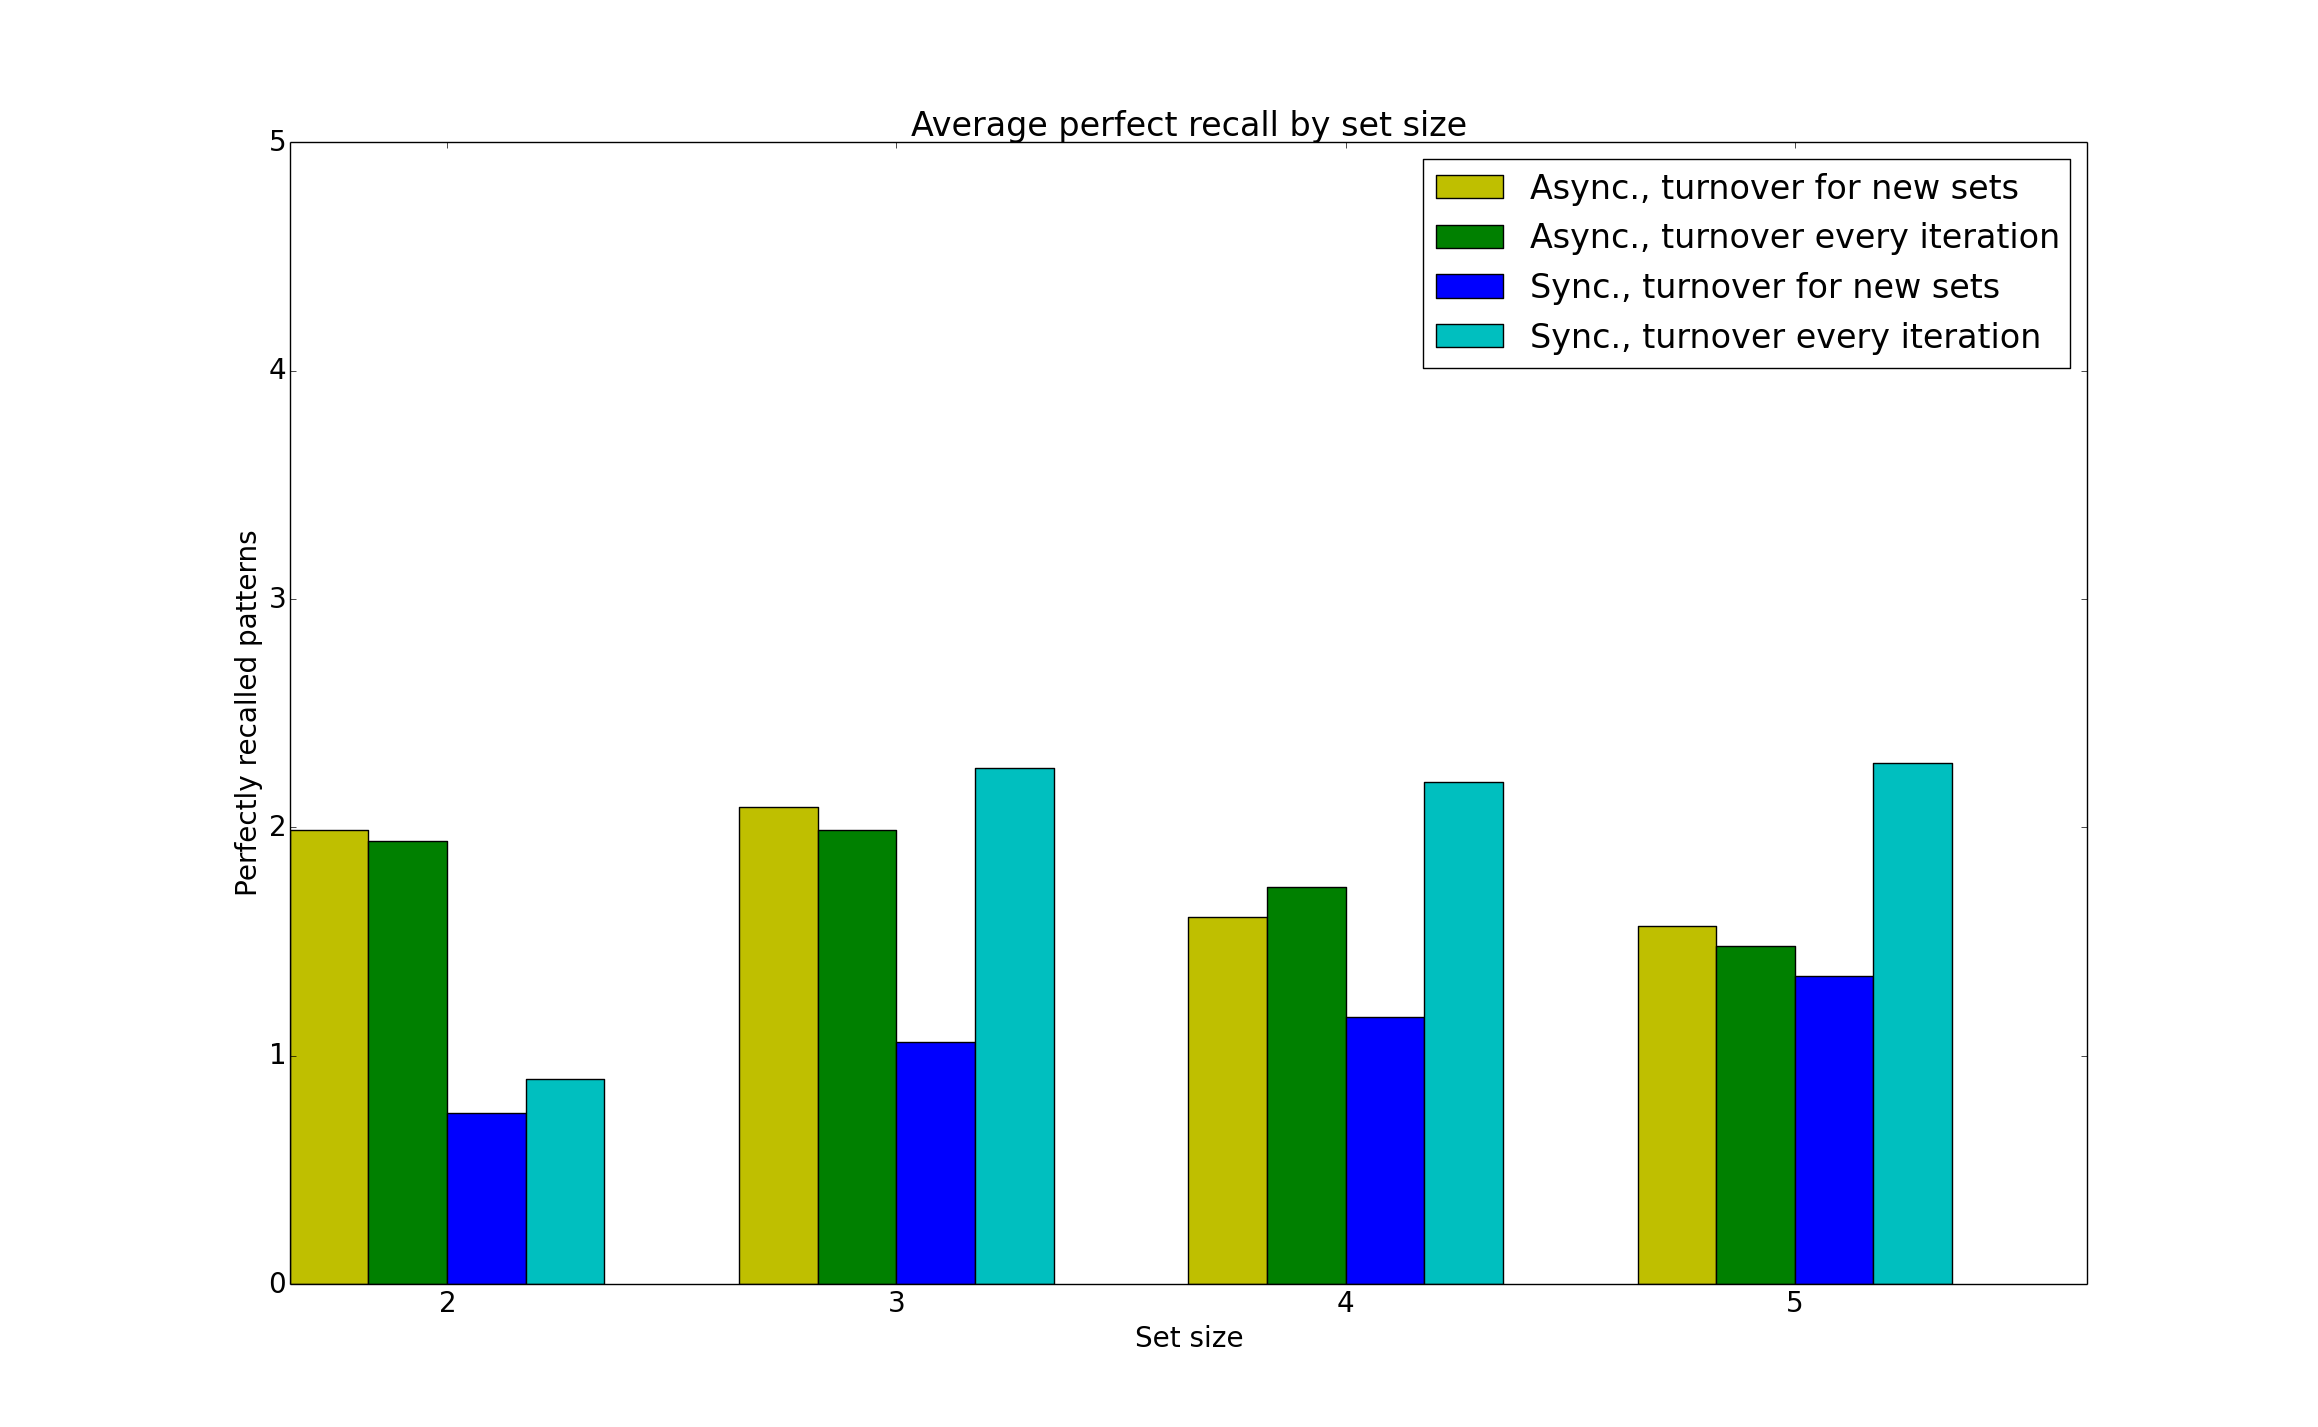
\includegraphics[width=13cm]{fig/avg_perfect_recall_bars.png}
    \caption{perf recall by set size bars}
    \label{fig:avg_perfect_recall_bars}
\end{figure}

\begin{figure}[h!]
    \centering
    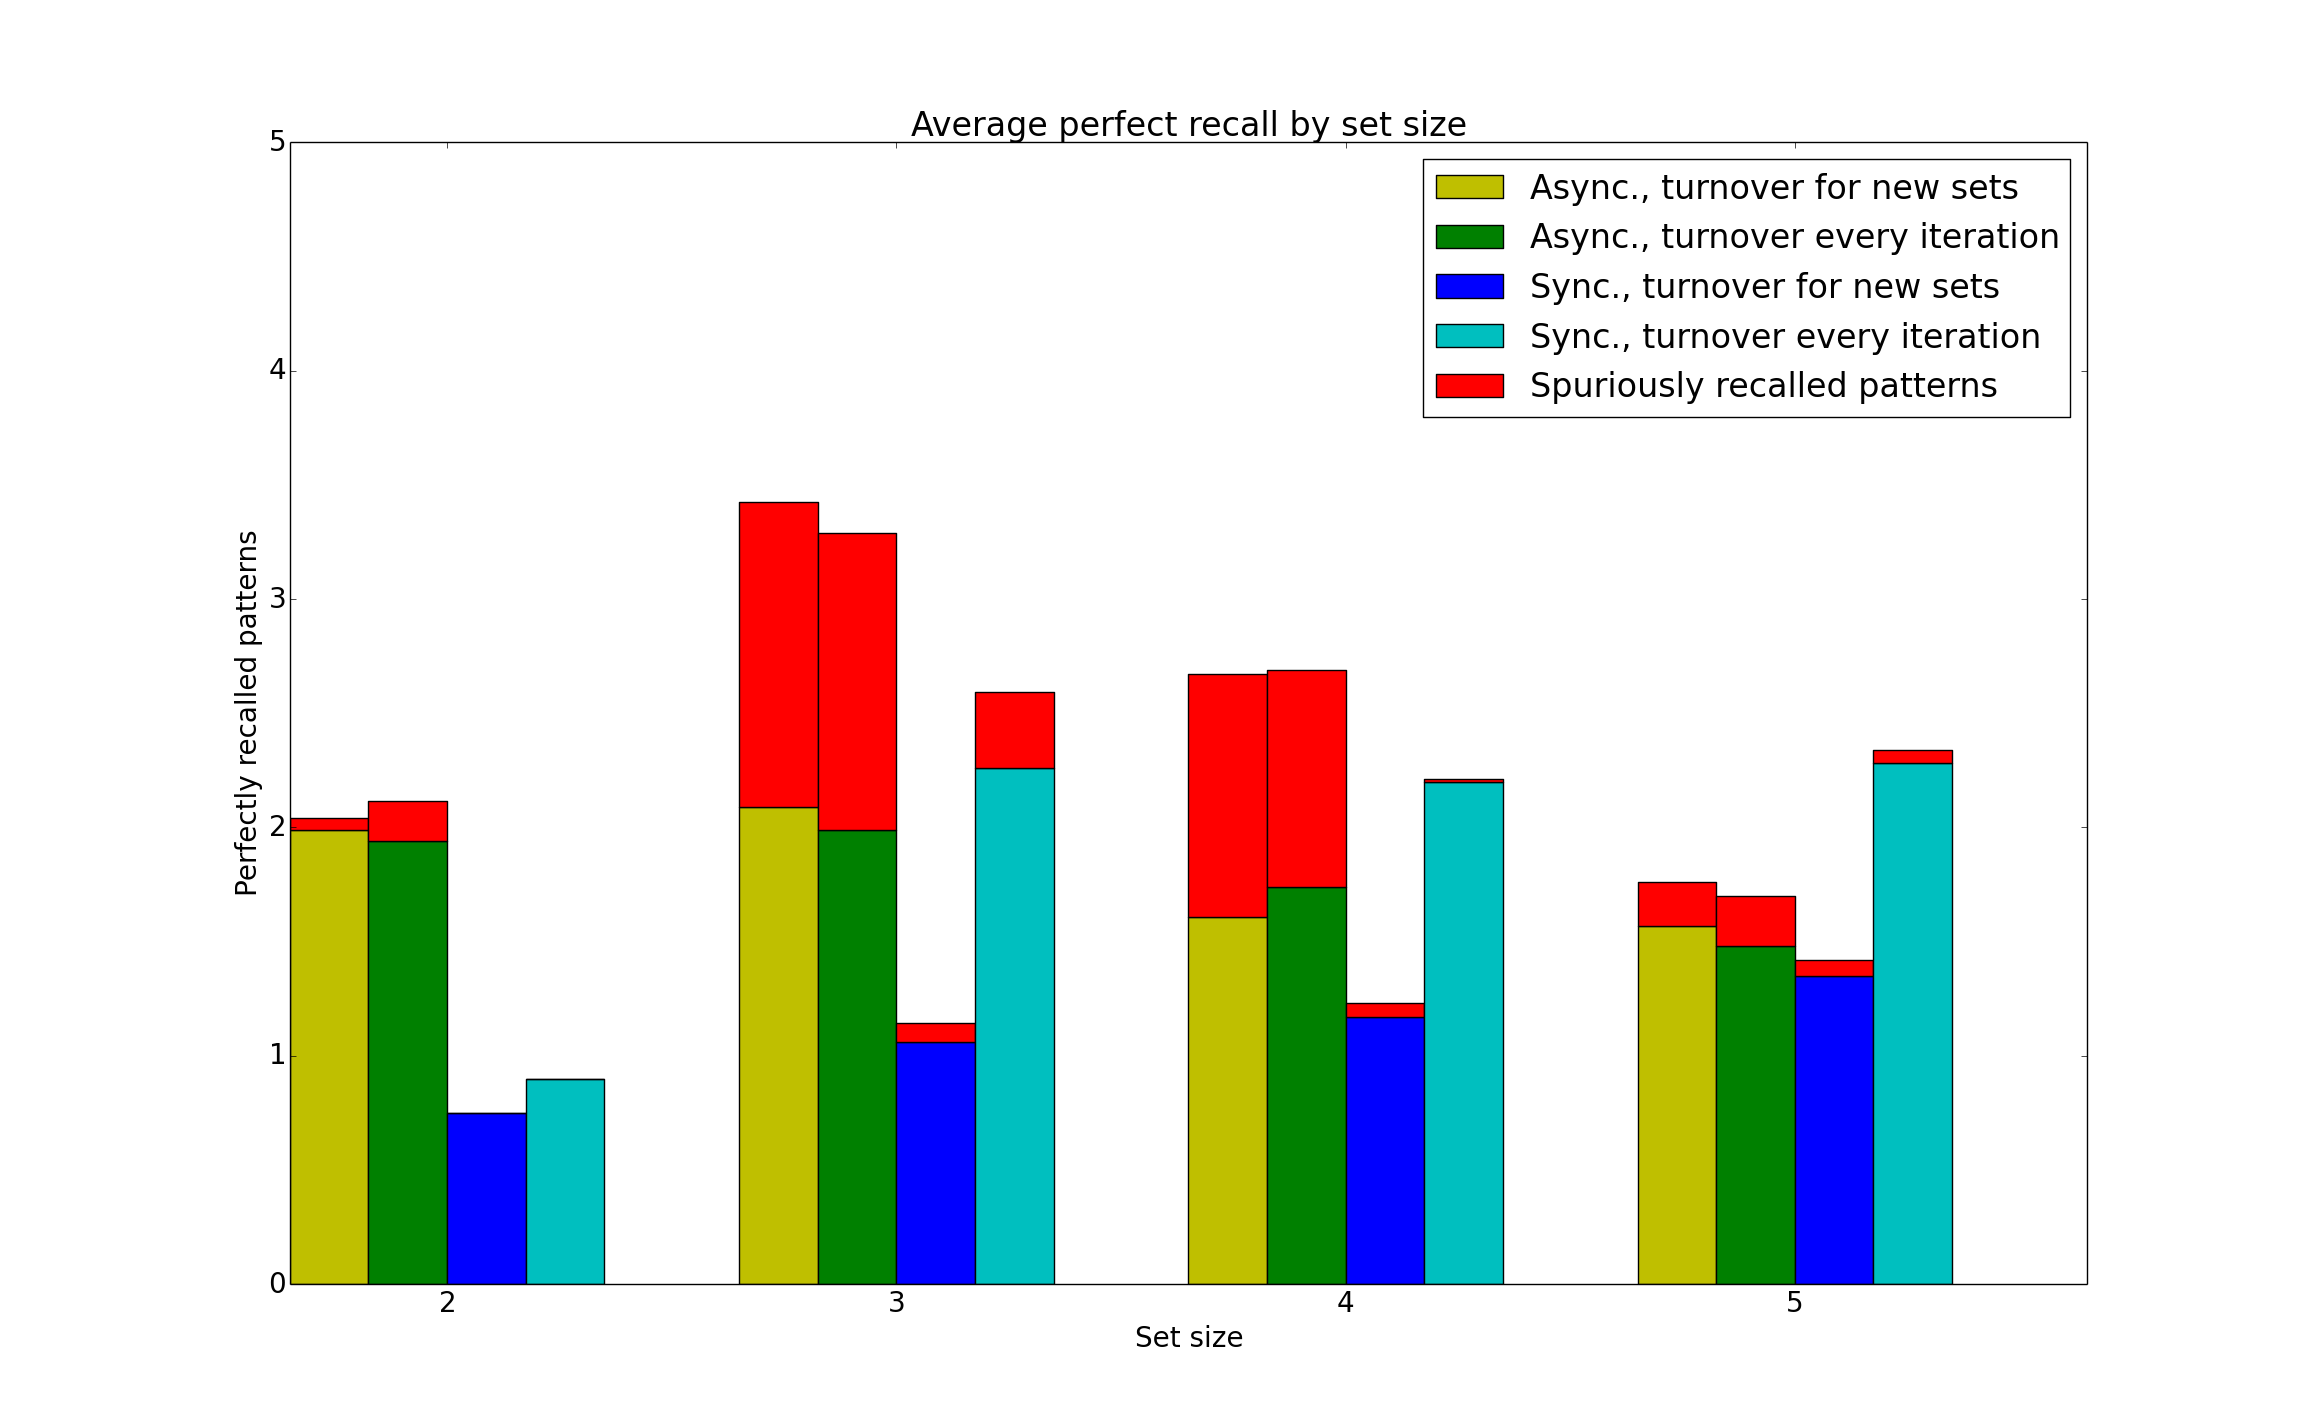
\includegraphics[width=13cm]{fig/avg_perfect_recall_rates_with_spurious_bars.png}
    \caption{perf recall by set size bars with spurious}
    \label{fig:avg_perfect_recall_rates_with_spurious_bars}
\end{figure}

\begin{figure}[h!]
    \centering
    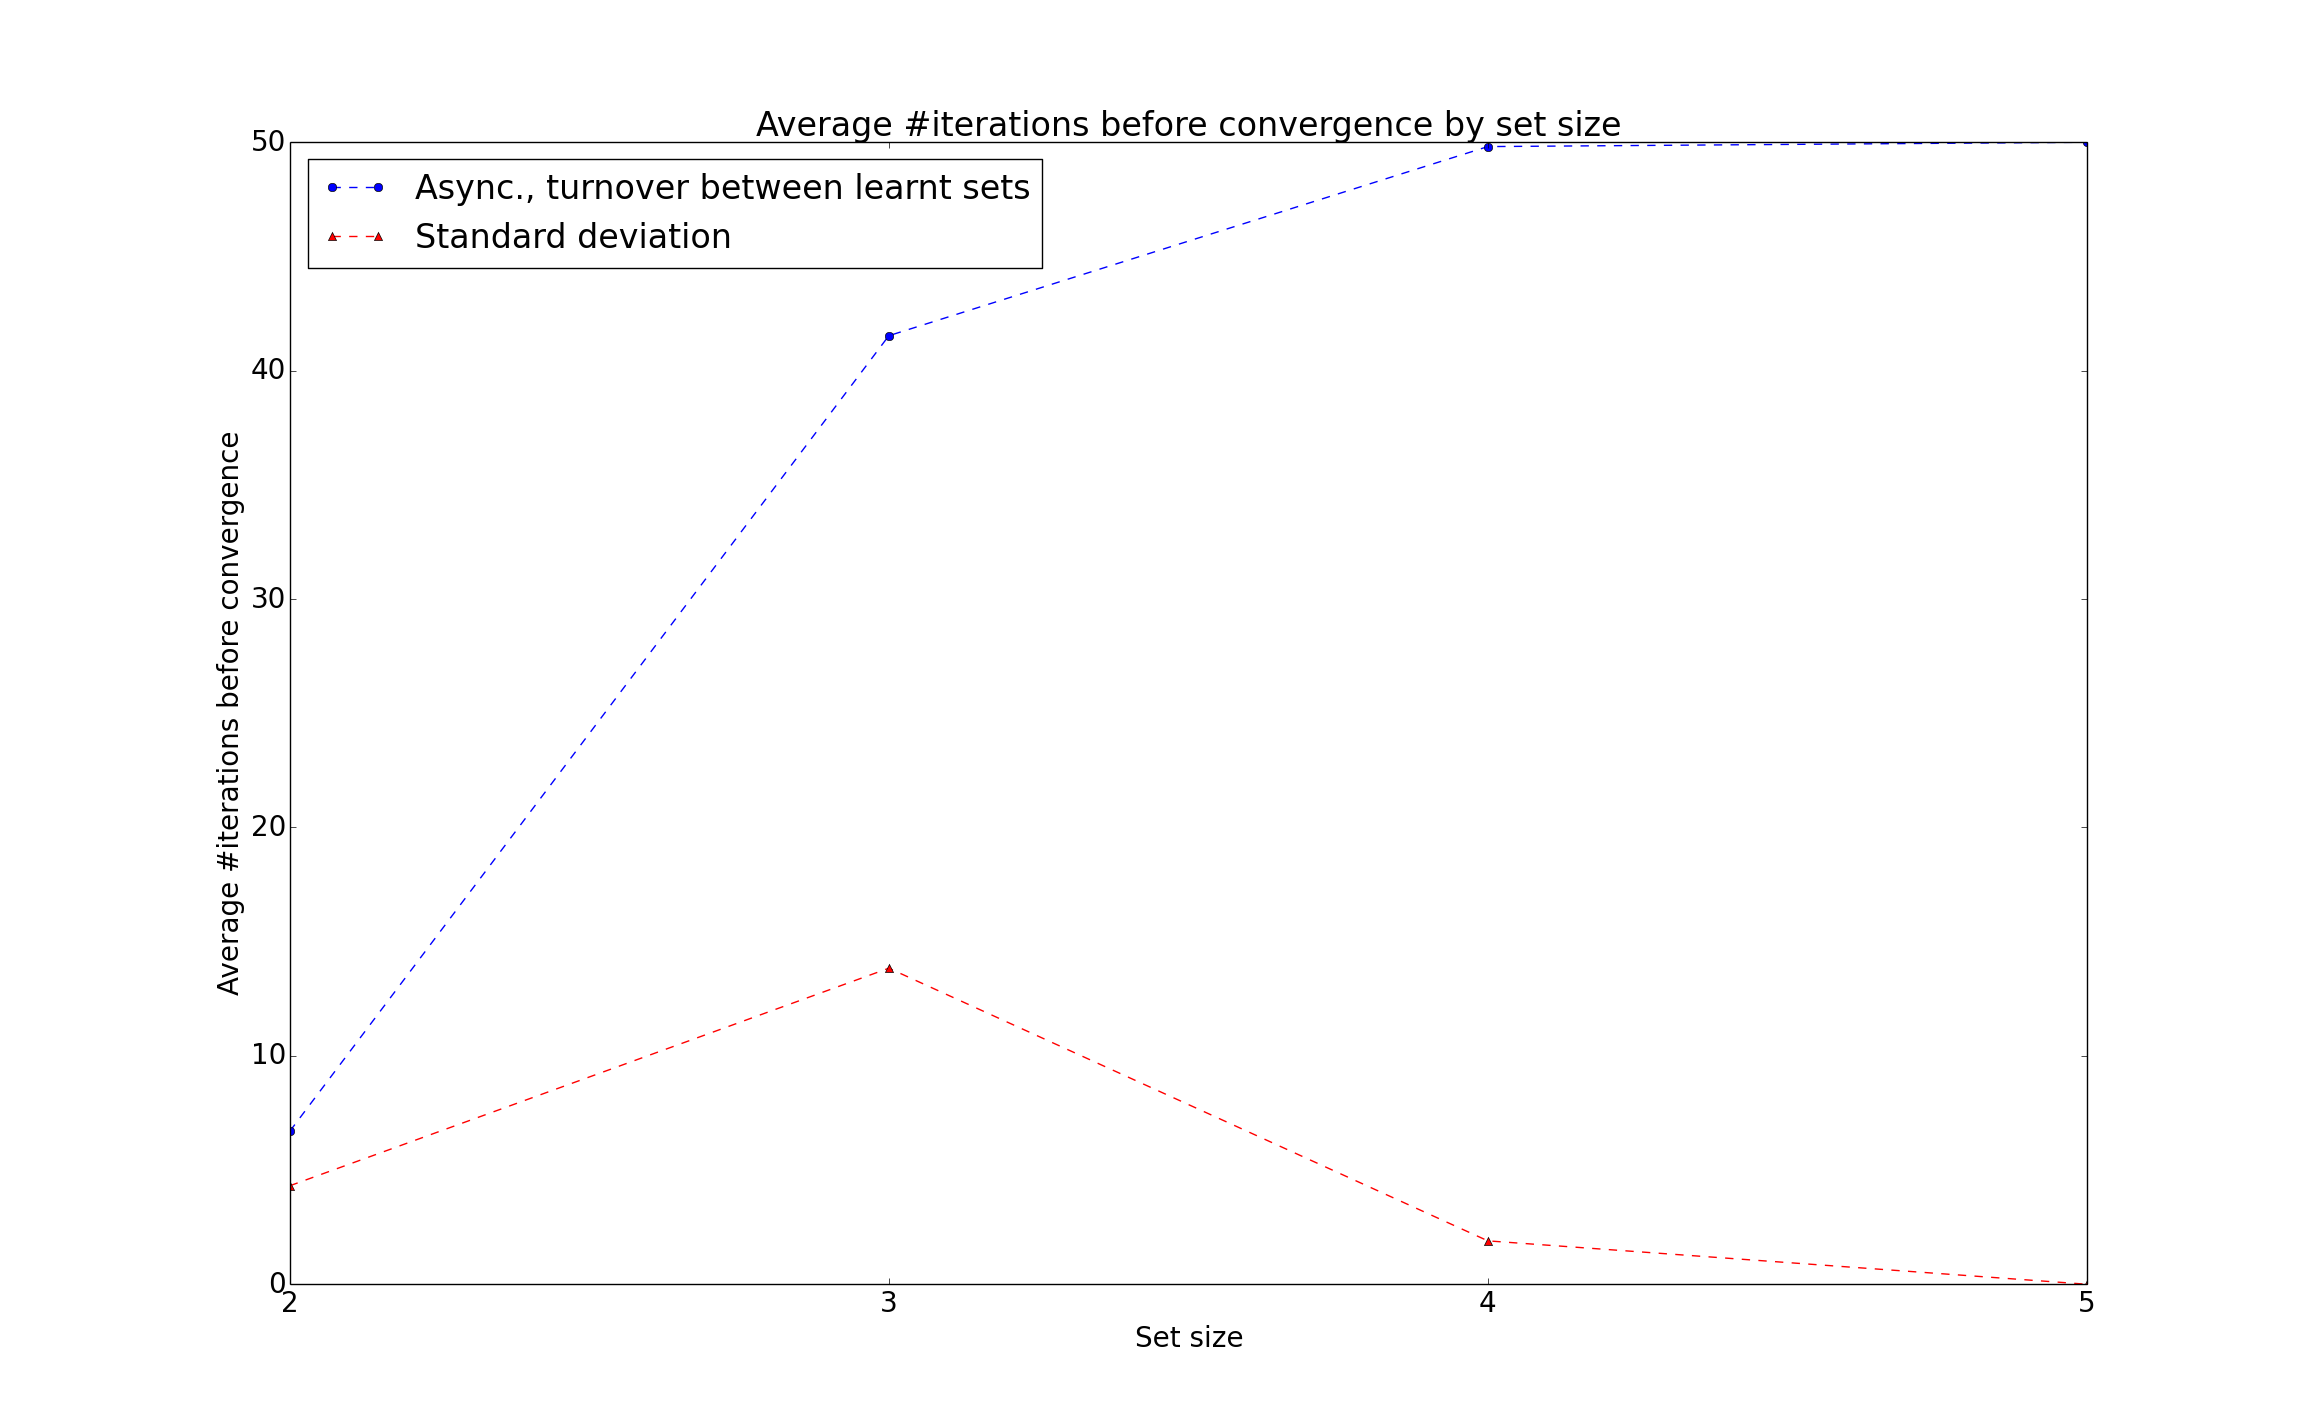
\includegraphics[width=13cm]{fig/avg_convergence_iterations_async_true_mode_0.png}
    \caption{avg iters to convergence, most successful; async true mode 0}
    \label{fig:avg_convergence_iterations_async_true_mode_0}
\end{figure}

\begin{figure}[h!]
    \centering
    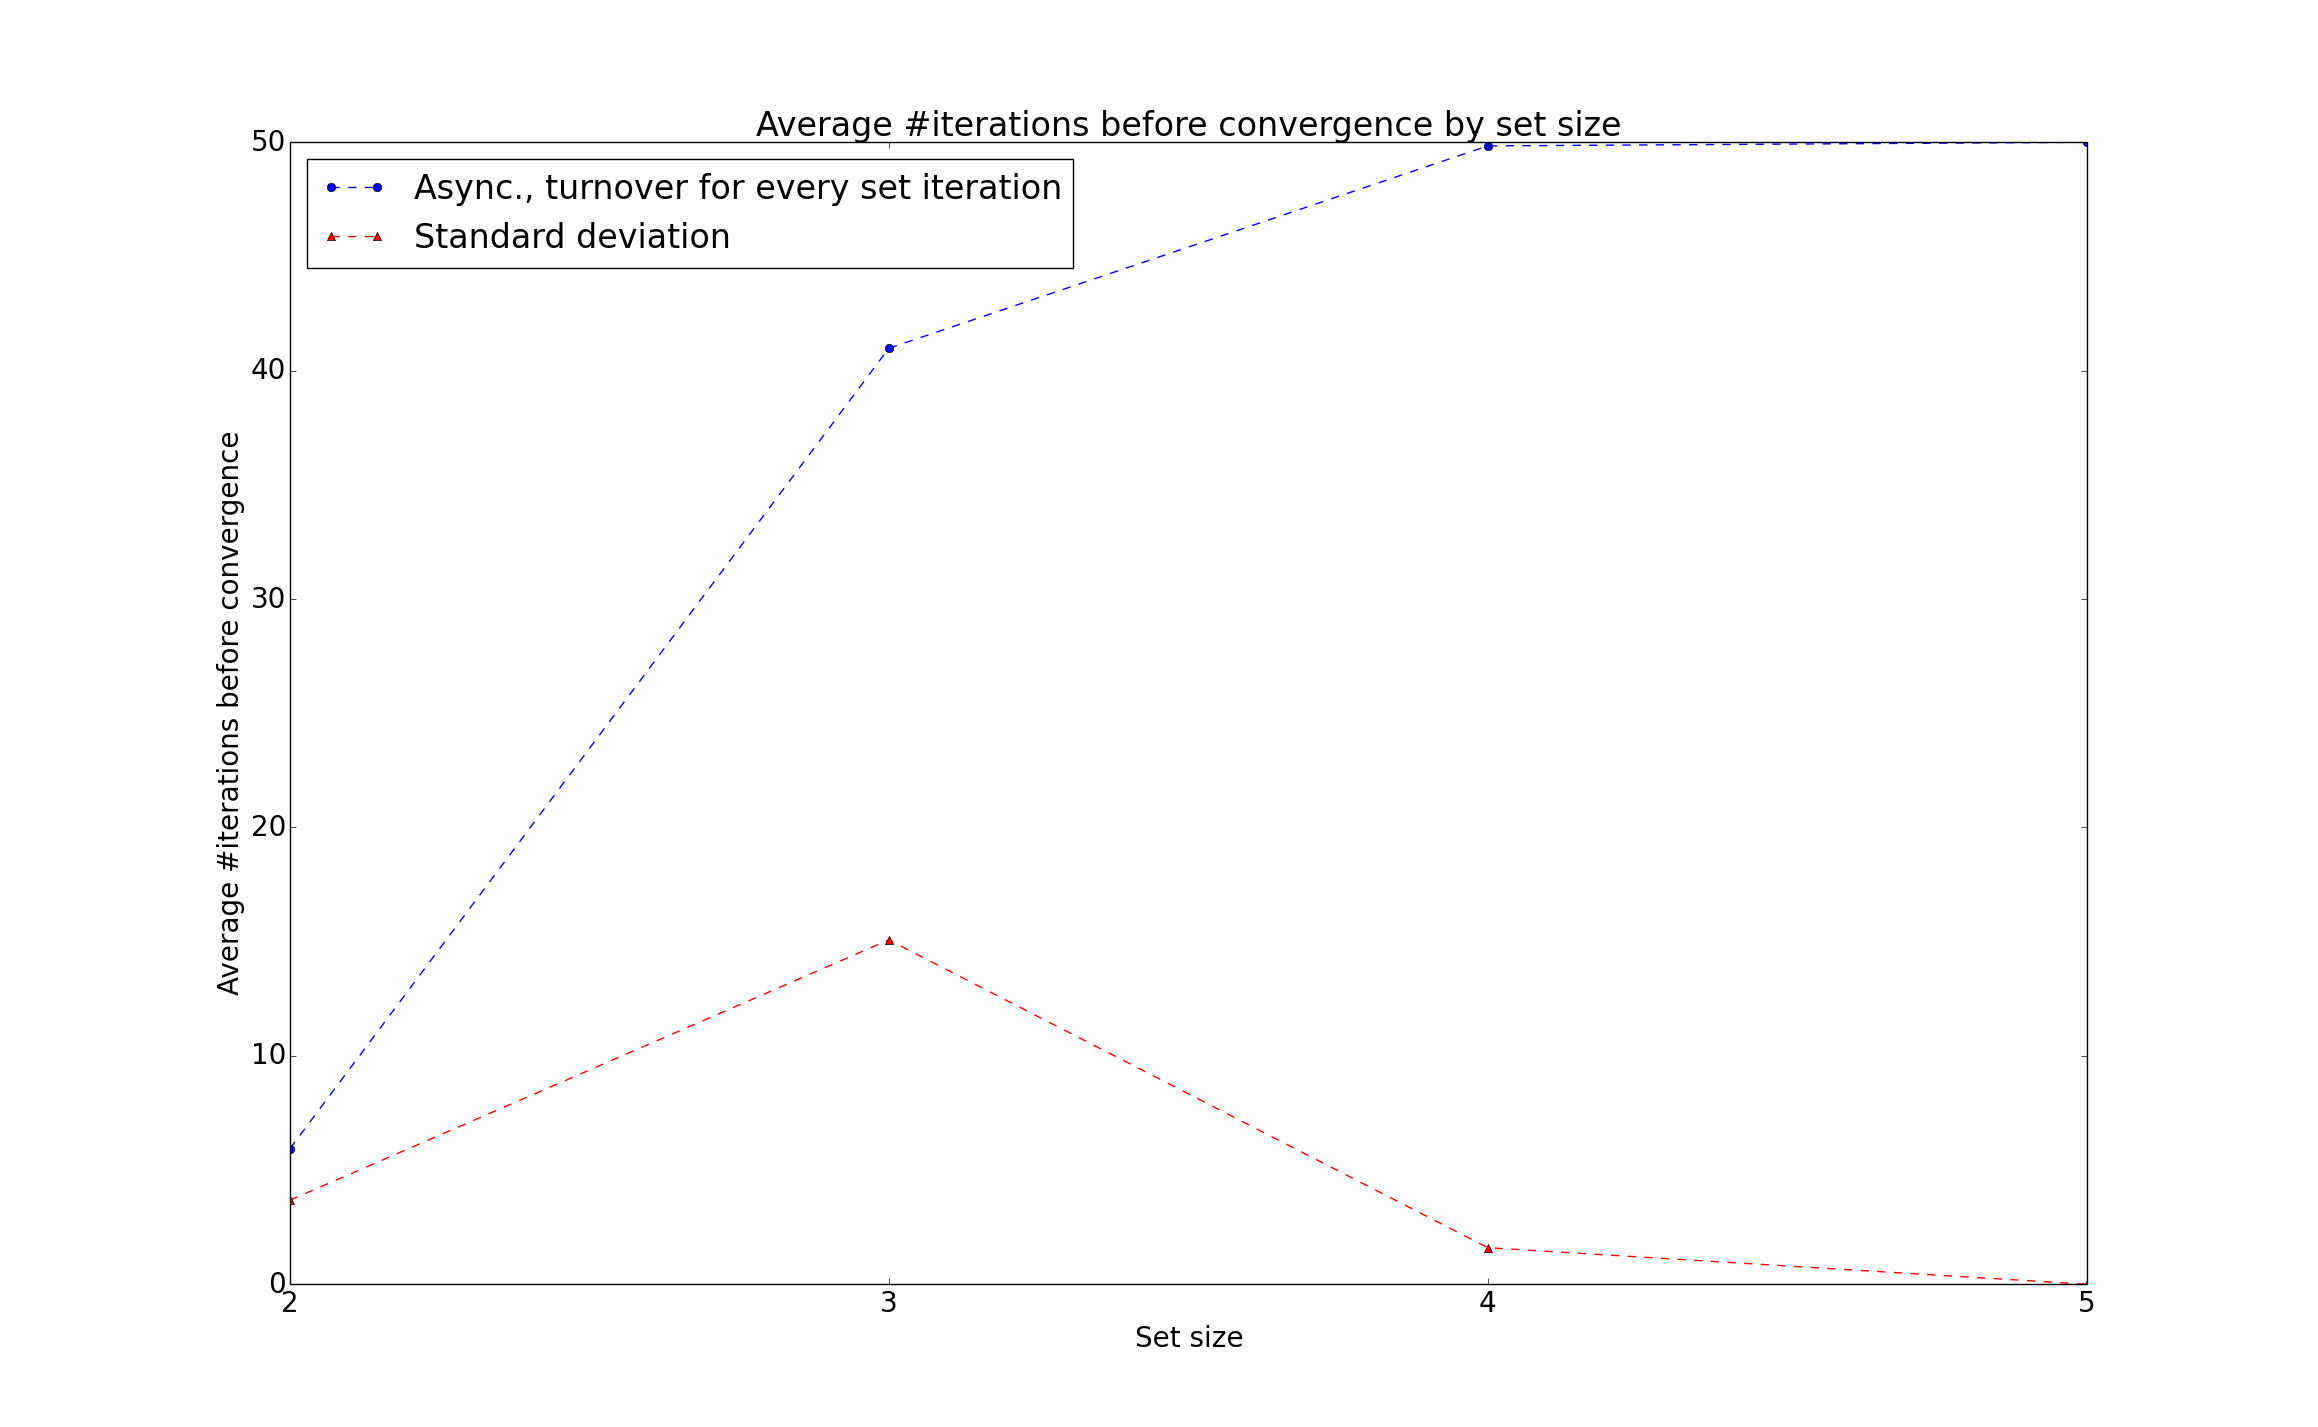
\includegraphics[width=13cm]{fig/avg_convergence_iterations_async_true_mode_1.png}
    \caption{avg iters to convergence, most successful; async true mode 1}
    \label{fig:avg_convergence_iterations_async_true_mode_1}
\end{figure}

\begin{figure}[h!]
    \centering
    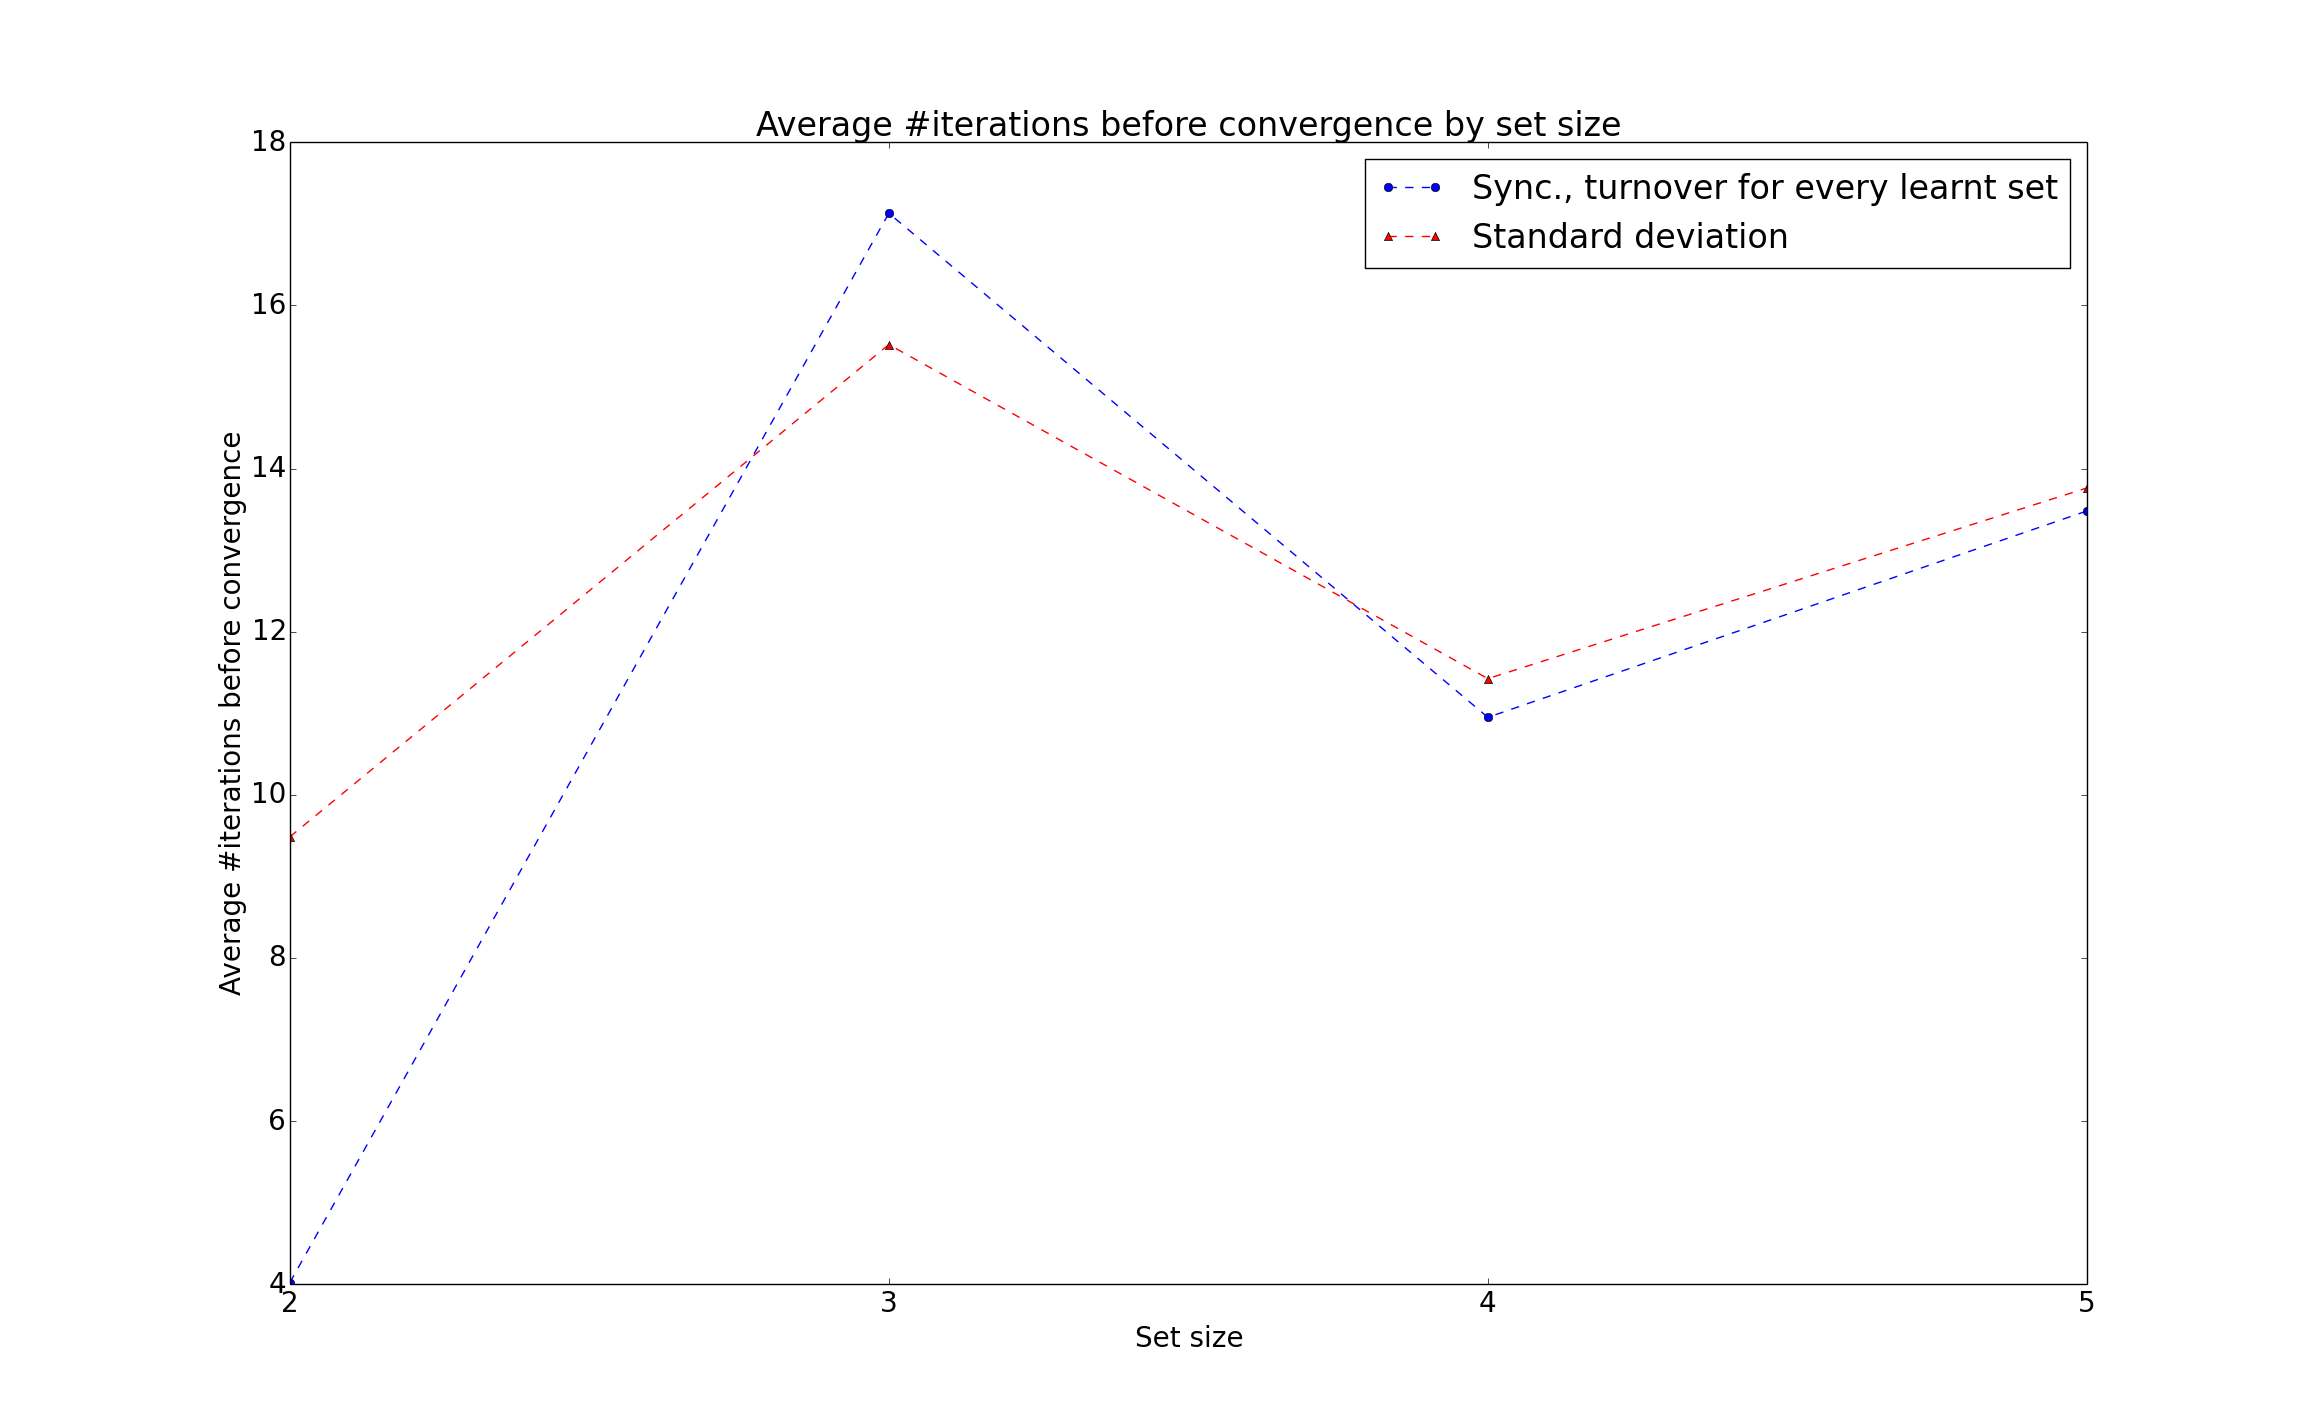
\includegraphics[width=13cm]{fig/avg_convergence_iterations_sync_mode_0.png}
    \caption{avg iters to convergence, most successful; sync mode 0}
    \label{fig:avg_convergence_iterations_sync_mode_0}
\end{figure}

\begin{figure}[h!]
    \centering
    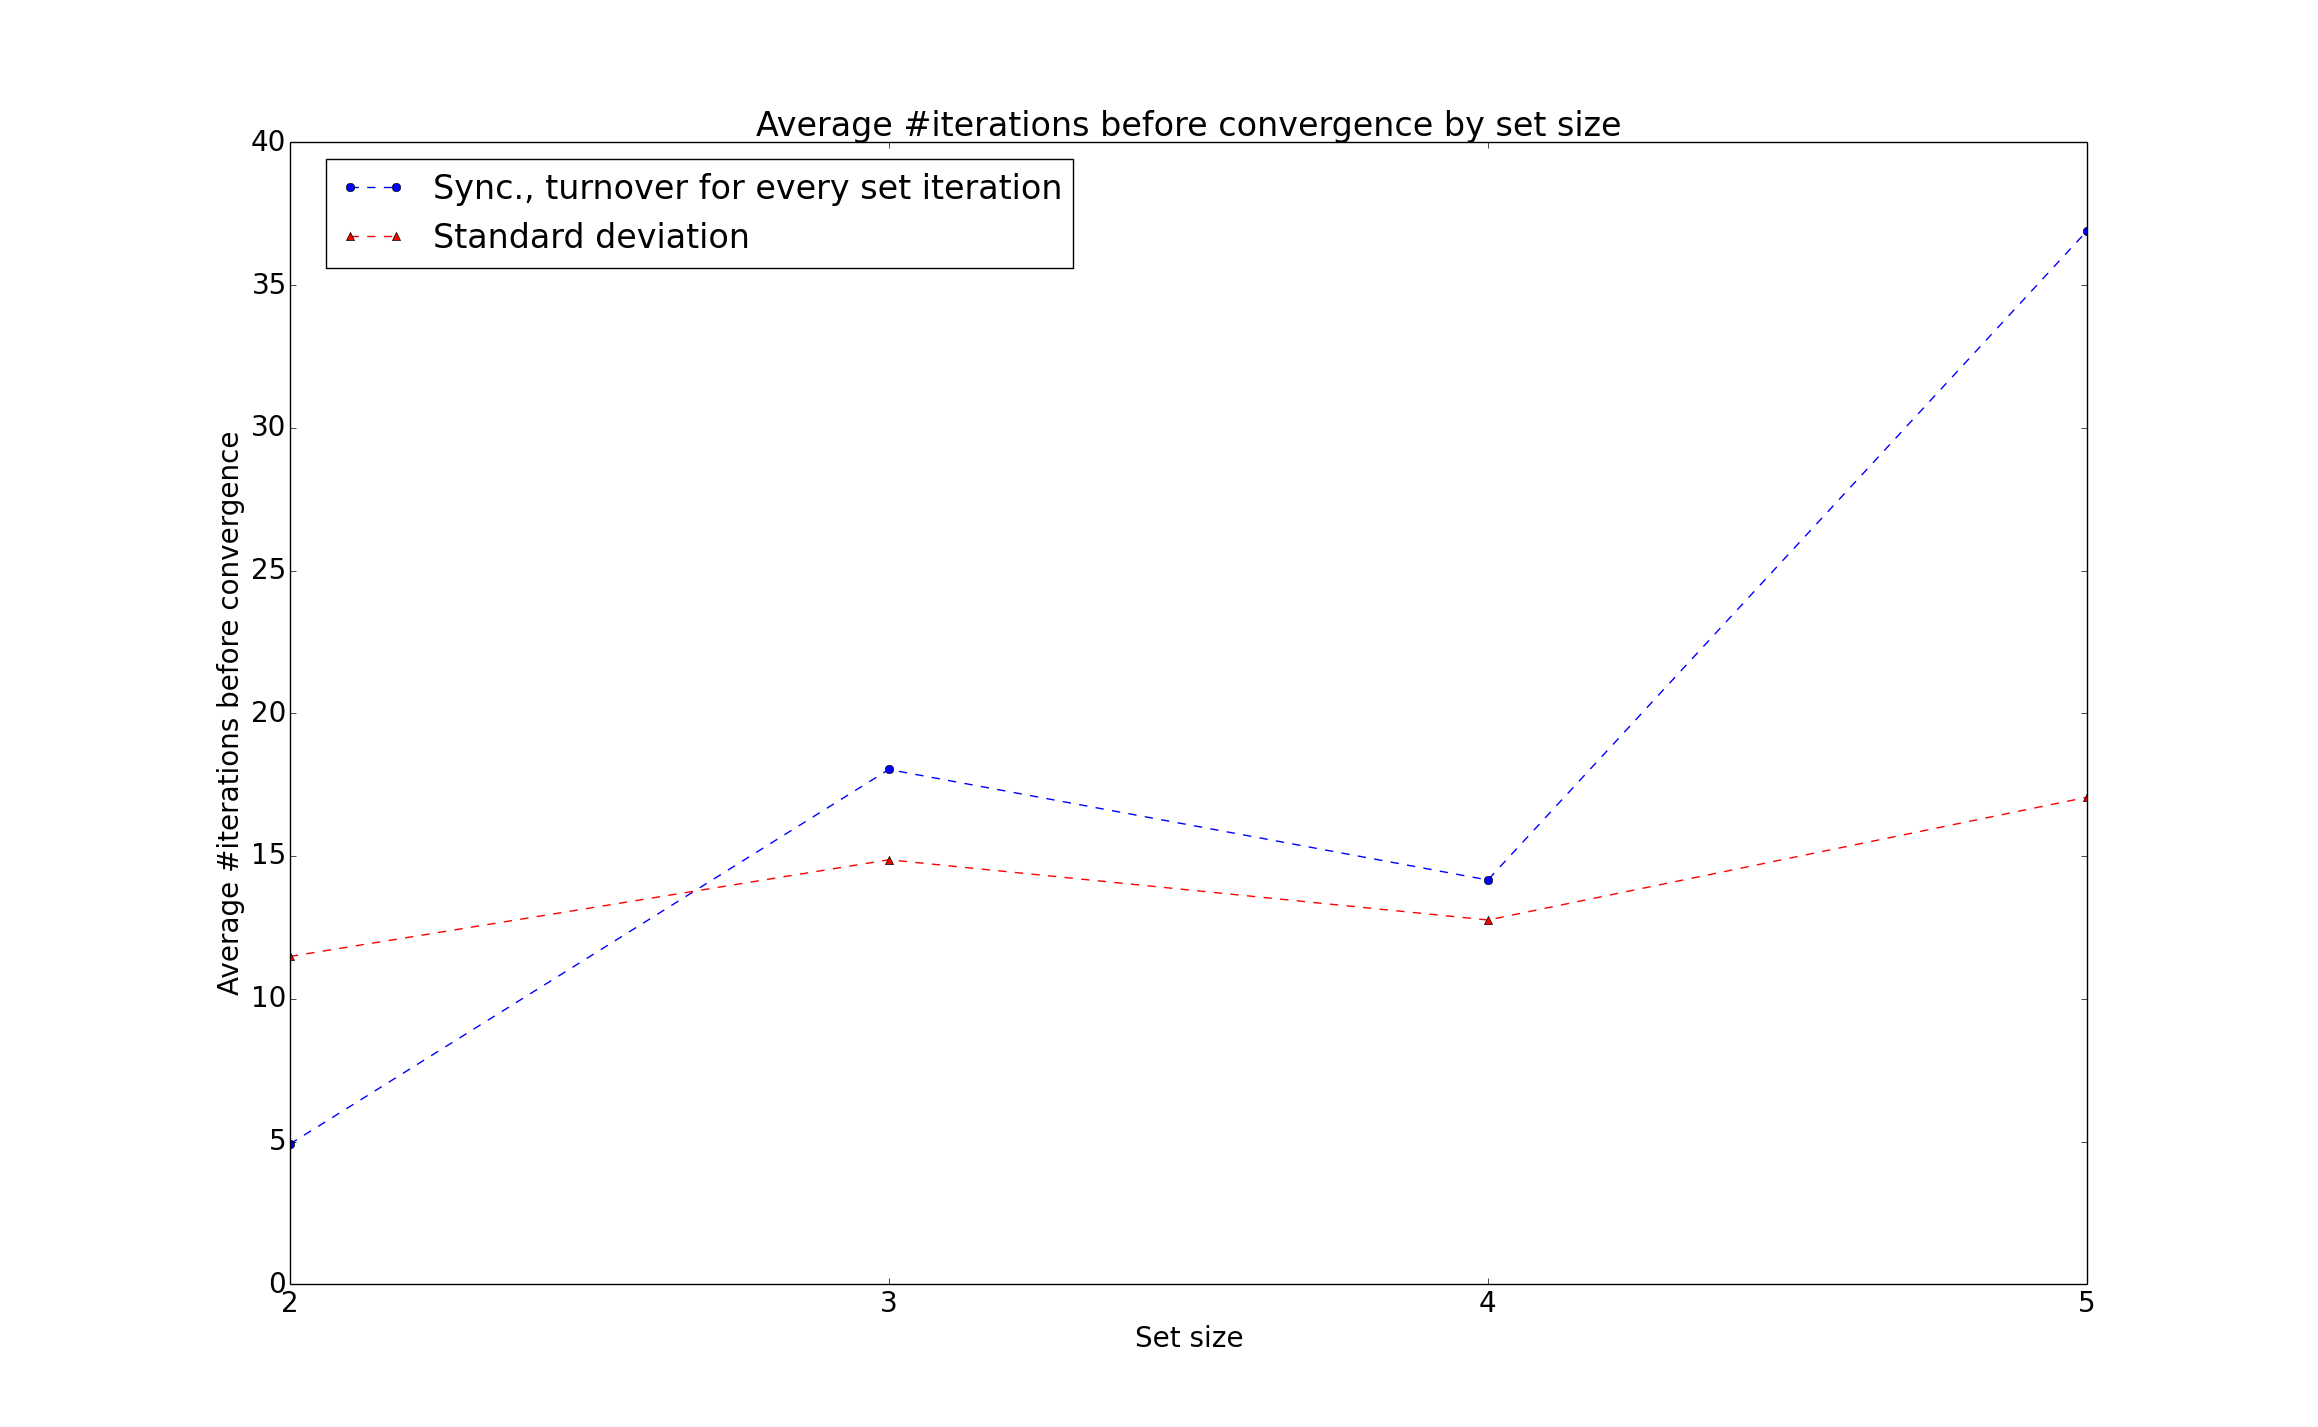
\includegraphics[width=13cm]{fig/avg_convergence_iterations_sync_mode_1.png}
    \caption{avg iters to convergence, most successful; sync mode 1}
    \label{fig:avg_convergence_iterations_sync_mode_1}
\end{figure}

\begin{figure}[h!]
    \centering
    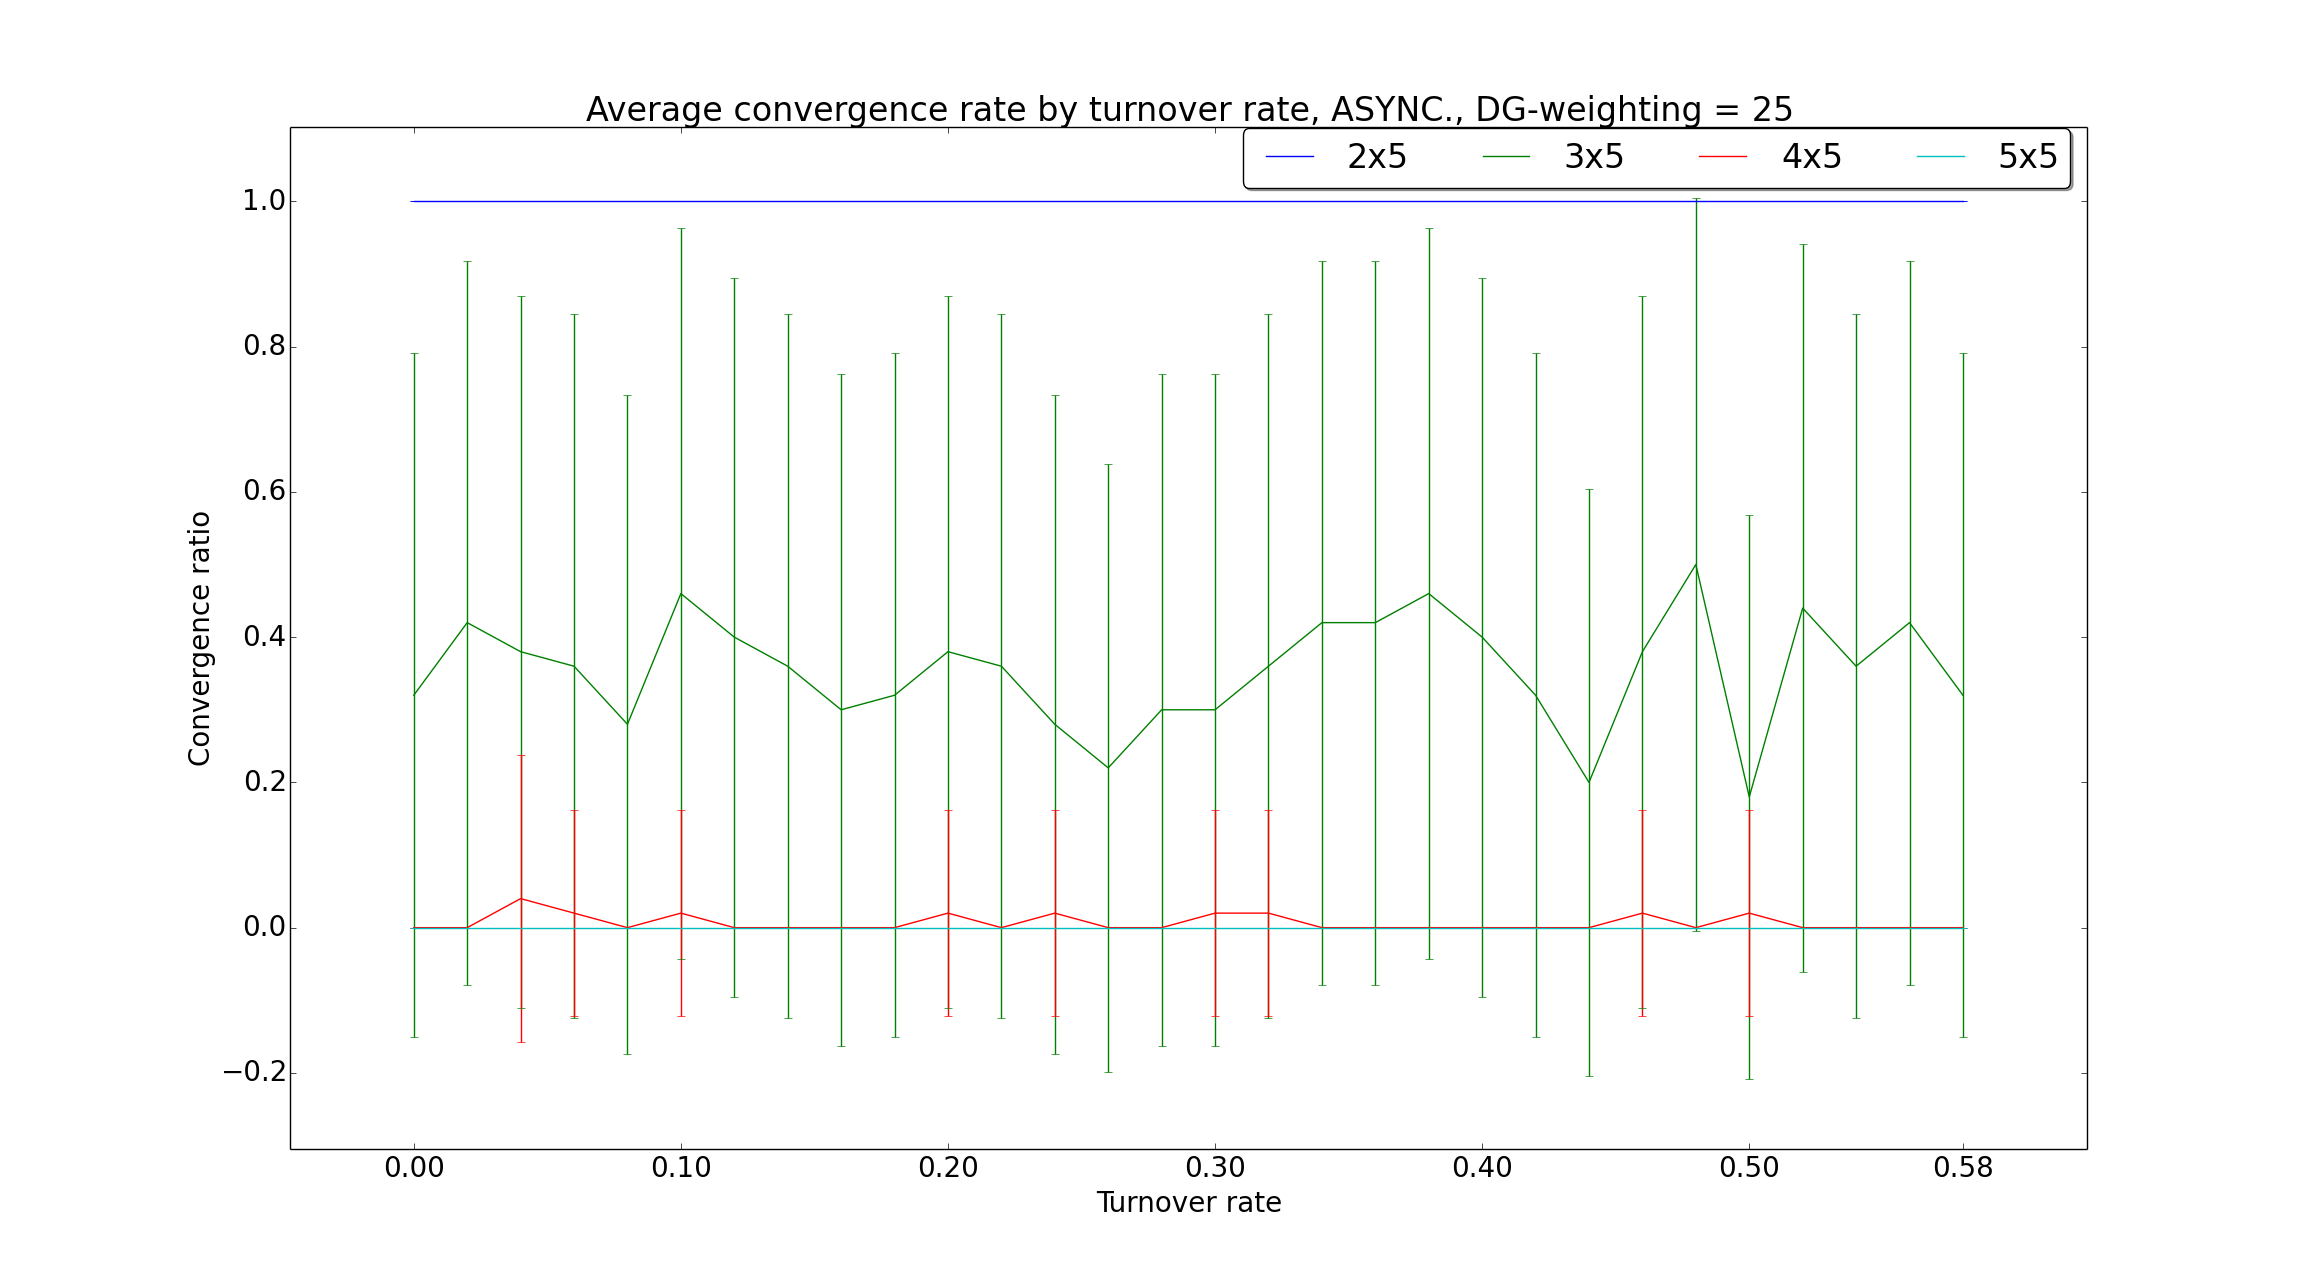
\includegraphics[width=13cm]{fig/avg_convergence_by_turnover_rate_async_dgw_25.png}
    \caption{avg convergence by turnover rate, async, dgw 25. note that it does not seem to impact this configuration - possibly async altogether. need to analyse changing the turnover rate for dgw 1, and also dgw for turnover rate 0.5 and 0.04}
    \label{fig:avg_convergence_by_turnover_rate_async_dgw_25}
\end{figure}

\begin{figure}[h!]
    \centering
    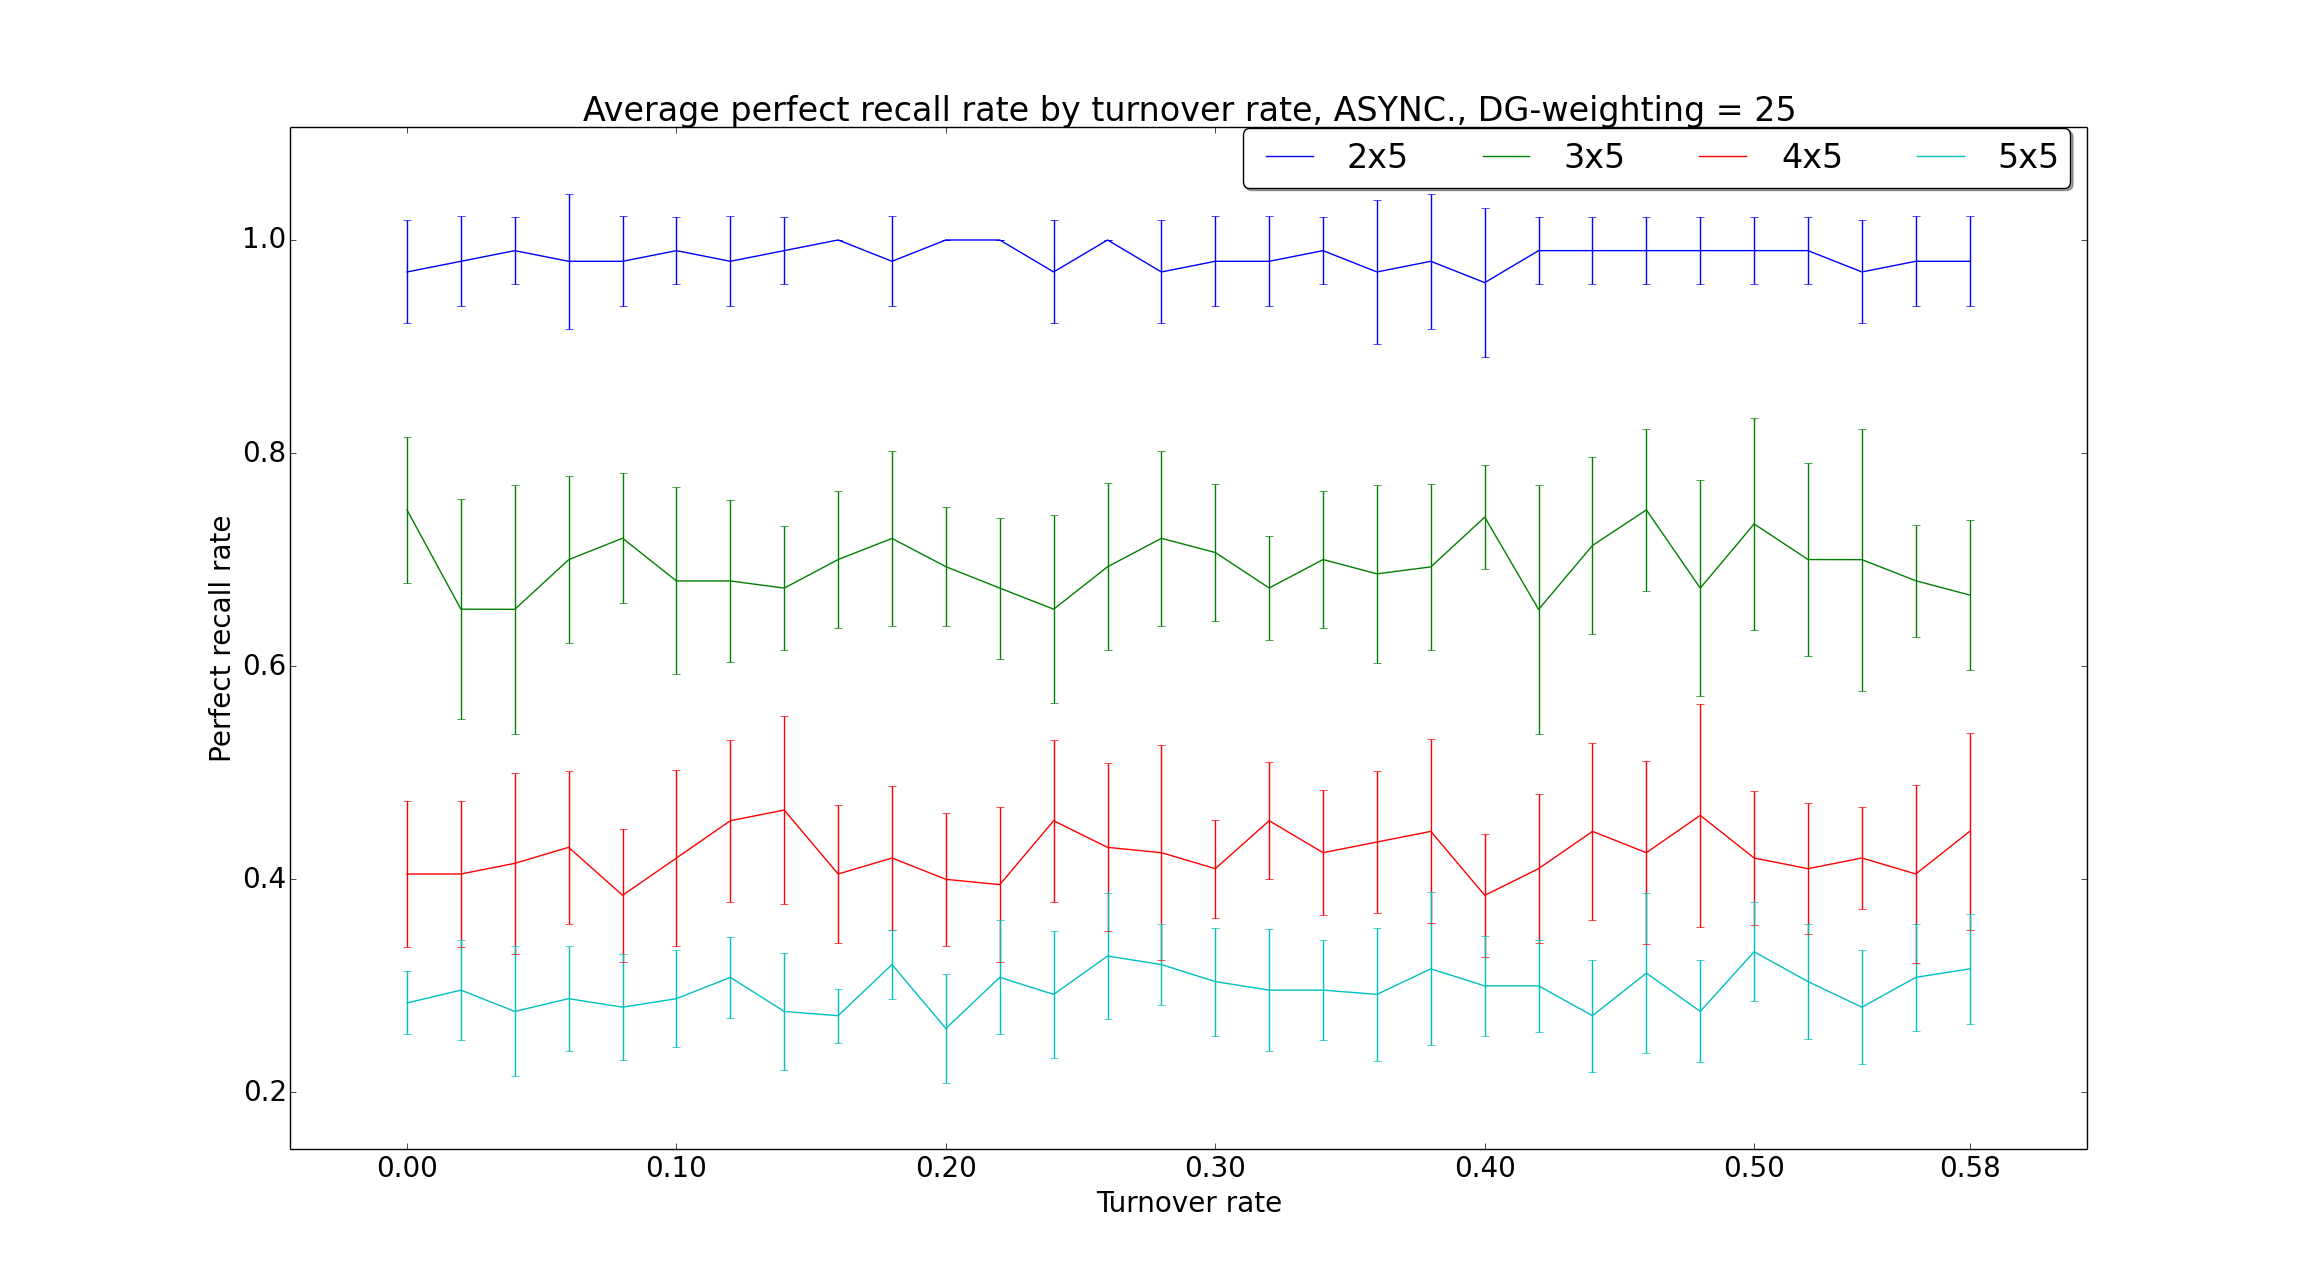
\includegraphics[width=13cm]{fig/avg_perfect_recall_rate_by_turnover_rate_async_dgw_25.png}
    \caption{avg perfect recall rate by turnover rate. note that it does not seem to impact the p.r.r. - see figure above. possibly async removes the impact this may have, although not successfully separating the given patterns - though increasing perfect recall for smaller set sizes when successful separation occurs.}
    \label{fig:avg_perfect_recall_rate_by_turnover_rate_async_dgw_25}
\end{figure}

\subsection{Experiment 2: Hippocampal model calibration}
\subsubsection{Methods}
\subsubsection{Results}

\subsection{Experiment 3: Extracting auto-associative patterns by chaotic recall}
\subsection{Experiment 4: Extracting hetero-associative patterns by chaotic recall}

\subsection{Experiment 5: Consolidation performance, experiment 3}
\subsection{Experiment 6: Consolidation performance, experiment 4}

\subsection{Experiment Y: Novel}


% ========================== RESULTS ============================
\section{Results}
some patterns may be recalled after the next training set has been learned. i allowed this to put the pattern in the set of chaotically recalled patterns, because it reflects something which is fairly stable in the hippocampal module.
\\

Async. seems to be by far the most accurate in terms of perfect recall when it converges. Sync. with turnover for every learnt set has the highest convergence rate - non-changing for different set sizes, but the worst perfect recall rate.

It would be very interesting to see how using the 'spurious' patterns along with the actual matching patterns would consolidate to the neocortical network, comparing this to the performance attained by using the formerly outlined pseudopattern generation. In the event of having a similar effect from pattern consolidation using spurious patterns, this may point in the direction of spontaneously generated 'spurious' patterns in fact possibly acting as pseudopatterns, thus outlining a process for pseudopattern generation in the brain. (Where the stability during recall could determine the consolidation strength. For complete convergence during training using async, mode 0, about 7 iterations were required for convergence - which is thought to be (?) the number of required iterations for successful neocortical memory consolidation. This could be a spurious correlation - however, the number is equal during convergence for set size 2. If the same number of iteration can be required for a successful configuration for set size 3, this would suggest that the number is not spurious.)
\\

Along with the spurious patterns, if considering the sum of distinct perfectly recalled patterns and spurious patterns as containing information about the number of patterns, the asynchronous scheme seems to contain the most information, only falling off at set size 5. This is most likely due to the convergence being 0 \% , which it actually is at set size 4, too. Increasing the number of iterations may remedy this - however, a further calibration is most likely more relevant.
\\

The recall rate is much better for the same convergence rate in the asynchronous scheme, which points towards this being the preferable scheme. Furthermore, because turnover for every set iteration remains biologically implausible, a more plausible, yet still unrealistic model should be chosen. I.e. Async., turnover for every new set.

STD only log() in async. -> points to more stable/realistic mechanism?
\\

Gradual exposure through the constant output of the HPC during recall and learning? If this may consolidate something to the PFC, it would be really interesting.
\\

In order to target the black-box analysis that analyzing an ANN can be - particularly for the case of biologically realistic networks using chaotic neurons - I employed a type of logging, from which data is parsed, and sorted by a parser that I wrote. This data includes the number of spurious patterns extracted, where spurious is defined as not perfectly overlapping any of the provided training patterns. Furthermore, it includes the number of iterations before convergence, where 50 iterations is considered as failure to converge. It also includes the weighting selected for the connections from the DG, the neuronal turnover rate that was employed, and lastly the number of extracted patterns, along with the perfect recall rate for the current experiment.


% ========================== section ============================
Experiment design
Results
Comparisons

\section*{Notes}

Enforce sparsity through weight updates corresponding only to the winners of kWTA - didn't work.

\textbf{100 \% connection ratio EC-CA3:}

Fairly rapid convergence for three patterns in HPC-module for turnover between every training set iteration. 
Not necessarily successful recall of all patterns. Does this have something to do with the synchronized CA3-layer during recall? Separation possible during recall when the desired pattern(s) are presented to the network - however, not all may be recalled.

-> New random pattern each time stability was reached resulted in better recall.

Is this also the case for heavier weighting of the DG-CA3 path during learning?

Spurious pattern reduction/correlation with occurrence when using turnover?

Convergence when turnover is removed between set iterations?

Heavier weighting DG. Based on paper \citep{Norman2003}. Empirical results. Chpt. 4. Figures. Nice.

\section*{Model calibration}

Experiments designed for model calibration

Dimensions analyzed outlined above.

First: STM-network extraction rate (at first, empirically observed to be same as solely auto-associative Hopfield network).


\textbf{Notes}

experiments suite - two as outlined by \citep{Hattori2014}, originally retrieved from ... as outlined above
enabling several trials automatically.

Turnover between every training set iteration (?). Needs to include empirical data on decision making. Move to preliminary experimentation in chpt. 4?

\cleardoublepage